\documentclass[twoside]{book}

% Packages required by doxygen
\usepackage{fixltx2e}
\usepackage{calc}
\usepackage{doxygen}
\usepackage[export]{adjustbox} % also loads graphicx
\usepackage{graphicx}
\usepackage[utf8]{inputenc}
\usepackage{makeidx}
\usepackage{multicol}
\usepackage{multirow}
\PassOptionsToPackage{warn}{textcomp}
\usepackage{textcomp}
\usepackage[nointegrals]{wasysym}
\usepackage[table]{xcolor}

% Font selection
\usepackage[T1]{fontenc}
\usepackage[scaled=.90]{helvet}
\usepackage{courier}
\usepackage{amssymb}
\usepackage{sectsty}
\renewcommand{\familydefault}{\sfdefault}
\allsectionsfont{%
  \fontseries{bc}\selectfont%
  \color{darkgray}%
}
\renewcommand{\DoxyLabelFont}{%
  \fontseries{bc}\selectfont%
  \color{darkgray}%
}
\newcommand{\+}{\discretionary{\mbox{\scriptsize$\hookleftarrow$}}{}{}}

% Page & text layout
\usepackage{geometry}
\geometry{%
  a4paper,%
  top=2.5cm,%
  bottom=2.5cm,%
  left=2.5cm,%
  right=2.5cm%
}
\tolerance=750
\hfuzz=15pt
\hbadness=750
\setlength{\emergencystretch}{15pt}
\setlength{\parindent}{0cm}
\setlength{\parskip}{3ex plus 2ex minus 2ex}
\makeatletter
\renewcommand{\paragraph}{%
  \@startsection{paragraph}{4}{0ex}{-1.0ex}{1.0ex}{%
    \normalfont\normalsize\bfseries\SS@parafont%
  }%
}
\renewcommand{\subparagraph}{%
  \@startsection{subparagraph}{5}{0ex}{-1.0ex}{1.0ex}{%
    \normalfont\normalsize\bfseries\SS@subparafont%
  }%
}
\makeatother

% Headers & footers
\usepackage{fancyhdr}
\pagestyle{fancyplain}
\fancyhead[LE]{\fancyplain{}{\bfseries\thepage}}
\fancyhead[CE]{\fancyplain{}{}}
\fancyhead[RE]{\fancyplain{}{\bfseries\leftmark}}
\fancyhead[LO]{\fancyplain{}{\bfseries\rightmark}}
\fancyhead[CO]{\fancyplain{}{}}
\fancyhead[RO]{\fancyplain{}{\bfseries\thepage}}
\fancyfoot[LE]{\fancyplain{}{}}
\fancyfoot[CE]{\fancyplain{}{}}
\fancyfoot[RE]{\fancyplain{}{\bfseries\scriptsize Generated by Doxygen }}
\fancyfoot[LO]{\fancyplain{}{\bfseries\scriptsize Generated by Doxygen }}
\fancyfoot[CO]{\fancyplain{}{}}
\fancyfoot[RO]{\fancyplain{}{}}
\renewcommand{\footrulewidth}{0.4pt}
\renewcommand{\chaptermark}[1]{%
  \markboth{#1}{}%
}
\renewcommand{\sectionmark}[1]{%
  \markright{\thesection\ #1}%
}

% Indices & bibliography
\usepackage{natbib}
\usepackage[titles]{tocloft}
\setcounter{tocdepth}{3}
\setcounter{secnumdepth}{5}
\makeindex

% Hyperlinks (required, but should be loaded last)
\usepackage{ifpdf}
\ifpdf
  \usepackage[pdftex,pagebackref=true]{hyperref}
\else
  \usepackage[ps2pdf,pagebackref=true]{hyperref}
\fi
\hypersetup{%
  colorlinks=true,%
  linkcolor=blue,%
  citecolor=blue,%
  unicode%
}

% Custom commands
\newcommand{\clearemptydoublepage}{%
  \newpage{\pagestyle{empty}\cleardoublepage}%
}

\usepackage{caption}
\captionsetup{labelsep=space,justification=centering,font={bf},singlelinecheck=off,skip=4pt,position=top}

%===== C O N T E N T S =====

\begin{document}

% Titlepage & ToC
\hypersetup{pageanchor=false,
             bookmarksnumbered=true,
             pdfencoding=unicode
            }
\pagenumbering{alph}
\begin{titlepage}
\vspace*{7cm}
\begin{center}%
{\Large My Project }\\
\vspace*{1cm}
{\large Generated by Doxygen 1.8.13}\\
\end{center}
\end{titlepage}
\clearemptydoublepage
\pagenumbering{roman}
\tableofcontents
\clearemptydoublepage
\pagenumbering{arabic}
\hypersetup{pageanchor=true}

%--- Begin generated contents ---
\chapter{P\+AV -\/ P3\+: detección de pitch}
\label{md_README}
\Hypertarget{md_README}
Para descargar los ficheros de esta práctica, debe ir a la página principal del repositorio Git\+Hub, \href{https://github.com/albino-pav/P3}{\tt práctica 3}, y clickar en la caja verde situada a la derecha, justo encima del listado de ficheros del repositorio, con el nombre $\ast$$\ast${\ttfamily Clone or download}$\ast$$\ast$. Al hacerlo, se despliega un menú en el que aparece la dirección del repositorio. Copie esta dirección en el portapapeles (puede usar la rata y {\bfseries \mbox{[}Ctrl-\/C\mbox{]}} o usar el icono a la derecha de la dirección). A continuación, vaya al directorio {\bfseries P\+AV} de su ordenador y ejecute la orden siguiente\+:


\begin{DoxyCode}
usuario:~/PAV$ git clone dirección\_copiada
\end{DoxyCode}


Si todo ha funcionado correctamente, el repositorio se descargará en su ordenador y estará preparado para trabajar en él.

\paragraph*{Creación de una rama ({\itshape branch}).}

Lo primero que debe hacer es crear una rama nueva en su repositorio, ya que Git\+Hub no le permitirá actualizar la rama principal ({\bfseries master}) del proyecto. Utilice un nombre que le identifique personalmente (una posible elección es su nombre y apellido). Si, como se recomienda, va a trabajar colaborativamente en el seno de su grupo de prácticas, es conveniente que uno de sus miembros escoja como nombre de la rama la combinación de los primeros apellidos de los integrantes del grupo.


\begin{DoxyCode}
usuario:~/PAV/P3$ git branch Fulano-Mengano
\end{DoxyCode}


\paragraph*{Inicialización del trabajo colaborativo usando Git\+Hub.}

Seguramente sea un buen momento para crear un repositorio con su copia del proyecto en {\bfseries Git\+Hub}. De este modo, los distintos miembros del grupo podrán realizar sus cambios localmente y compartir sus avances en un sitio común y accesible.

Para ello, lo primero que debe hacer es, si no dispone de ella, crear una cuenta en Git\+Hub. El proceso para ello es bastante sencillo siguiendo las instrucciones proporciondas por el proio Git\+Hub. Al contrario que Git, Git\+Hub se gestiona completamente desde un entorno gráfico súmamente intuitivo. Además, está razonablemente documentado, tanto internamente, mediante sus \href{https://guides.github.com/}{\tt Guías de Git\+Hub}, como externamente, mediante multitud de tutoriales, guías y vídeos disponibles gratuitamente en internet.

Cree un repositorio vacío en su nueva cuenta de Git\+Hub (aunque no es estrictamente necesario, use el mismo nombre que la práctica\+: {\bfseries P3}). Obtenga la dirección de su nuevo repositorio vacío, y declárelo como origen remoto de su repositorio local\+:


\begin{DoxyCode}
usuario:~/PAV/P3$ git remote add origin dirección-repositorio-vacío
\end{DoxyCode}


A continuación, ya puede sincronizar su repositorio remoto con su copia local con la orden\+:


\begin{DoxyCode}
usuario:~/PAV/P3$ git push origin master
\end{DoxyCode}


\subsection*{Entrega de la práctica.}

La entrega de la práctica se hará mediante {\itshape pull requests}. Conforme se acerque la fecha de entrega, prevista para alrededor del 3 de noviembre de 2019, se informará del procedimiento con mayor detalle.

\subsection*{Acerca de este fichero, R\+E\+A\+D\+M\+E.\+md, y del lenguaje en que está escrito, Markdown.}

R\+E\+A\+D\+M\+E.\+md es un fichero de texto escrito con un formato denominado {\itshape {\bfseries markdown}}. La principal característica de este formato es que, manteniendo la legibilidad cuando se visualiza con herramientas en modo texto ({\ttfamily more}, {\ttfamily less}, editores varios, ...), permite amplias posibilidades de visualización con formato en una amplia gama de aplicaciones; muy notablemente, {\bfseries Git\+Hub}, {\bfseries Doxygen} y {\bfseries Facebook} (ciertamente, \+:eyes\+:).

Por ejemplo, {\itshape markdown} permite construir tablas como la siguiente, que muestra distintas opciones de resalte del texto\+:

\tabulinesep=1mm
\begin{longtabu} spread 0pt [c]{*{4}{|X[-1]}|}
\hline
\rowcolor{\tableheadbgcolor}\textbf{ modo texto }&\PBS\centering \textbf{ modo gráfico }&\textbf{ modo texto }&\PBS\centering \textbf{ modo gráfico  }\\\cline{1-4}
\endfirsthead
\hline
\endfoot
\hline
\rowcolor{\tableheadbgcolor}\textbf{ modo texto }&\PBS\centering \textbf{ modo gráfico }&\textbf{ modo texto }&\PBS\centering \textbf{ modo gráfico  }\\\cline{1-4}
\endhead
{\ttfamily $\ast$cursiva$\ast$} &\PBS\centering $\ast$cursiva$\ast$ &{\ttfamily \+\_\+cursiva\+\_\+} &\PBS\centering \+\_\+cursiva\+\_\+ \\\cline{1-4}
{\ttfamily $\ast$$\ast$negrita$\ast$$\ast$} &\PBS\centering $\ast$$\ast$negrita$\ast$$\ast$ &{\ttfamily \+\_\+\+\_\+negrita\+\_\+\+\_\+} &\PBS\centering \+\_\+\+\_\+negrita\+\_\+\+\_\+ \\\cline{1-4}
{\ttfamily $\ast$$\ast$$\ast$cursiva y negrita$\ast$$\ast$$\ast$}&\PBS\centering $\ast$$\ast$$\ast$cursiva y negrita$\ast$$\ast$$\ast$&{\ttfamily \+\_\+\+\_\+\+\_\+negrita y cursiva\+\_\+\+\_\+\+\_\+} &\PBS\centering \+\_\+\+\_\+\+\_\+negrita y cursiva\+\_\+\+\_\+\+\_\+ \\\cline{1-4}
{\ttfamily \+\_\+$\ast$$\ast$negrita y cursiva$\ast$$\ast$\+\_\+}&\PBS\centering \+\_\+\+\_\+$\ast$negrita y cursiva$\ast$\+\_\+\+\_\+&{\ttfamily \+\_\+\+\_\+$\ast$cursiva y negrita$\ast$\+\_\+\+\_\+}&\PBS\centering \+\_\+$\ast$$\ast$cursiva y negrita$\ast$$\ast$\+\_\+ \\\cline{1-4}
\end{longtabu}

\begin{DoxyItemize}
\item N\+O\+TA\+: {\bfseries Doxygen} no muestra correctamente el texto con formato de la tabla anterior. Sin embargo, otros programas, en particular, {\bfseries Git\+Hub}, sí lo hacen.
\end{DoxyItemize}

También permite los links, como el siguiente, que permite acceder a los elementos más importantes de la sintaxis de este formato desde la página de su creador, {\itshape John Gruber}\+: \href{https://daringfireball.net/projects/markdown/syntax}{\tt Sintaxis de Markdown}.

Algunas aplicaciones añaden ampliaciones específicas al lenguaje, los llamados {\itshape flavours} (aromas). Esto es, a la vez, una ventaja y un inconveniente, ya que, aunque muchas de ellas son realmente útiles, rompen la unidad del lenguaje e introducen incompatibilidades. Ahora bien, como todos ellos mantienen como referencia la legibilidad del fichero original en modo texto, las incompatibilidades no suelen traducirse en situaciones demasiado desastrosas. Entre los flavours más importantes para nosotros cabe destacar el \href{https://guides.github.com/features/mastering-markdown/}{\tt Markdown de Git\+Hub} o el \href{http://www.doxygen.nl/manual/markdown.html}{\tt Markdown de Doxygen}. 
\chapter{Namespace Index}
\section{Namespace List}
Here is a list of all documented namespaces with brief descriptions\+:\begin{DoxyCompactList}
\item\contentsline{section}{\hyperlink{namespaceupc}{upc} \\*Name space of U\+PC }{\pageref{namespaceupc}}{}
\end{DoxyCompactList}

\chapter{Hierarchical Index}
\section{Class Hierarchy}
This inheritance list is sorted roughly, but not completely, alphabetically\+:\begin{DoxyCompactList}
\item \contentsline{section}{upc\+:\+:Circular\+Index}{\pageref{classupc_1_1CircularIndex}}{}
\item \contentsline{section}{upc\+:\+:Digital\+Filter}{\pageref{classupc_1_1DigitalFilter}}{}
\item \contentsline{section}{ffft\+:\+:Dyn\+Array$<$ T $>$}{\pageref{classffft_1_1DynArray}}{}
\item \contentsline{section}{ffft\+:\+:Dyn\+Array$<$ Data\+Type $>$}{\pageref{classffft_1_1DynArray}}{}
\item \contentsline{section}{ffft\+:\+:Dyn\+Array$<$ ffft\+:\+:Osc\+Sin\+Cos $>$}{\pageref{classffft_1_1DynArray}}{}
\item \contentsline{section}{ffft\+:\+:Dyn\+Array$<$ long $>$}{\pageref{classffft_1_1DynArray}}{}
\item \contentsline{section}{ffft\+:\+:F\+F\+T\+Real$<$ DT $>$}{\pageref{classffft_1_1FFTReal}}{}
\item \contentsline{section}{upc\+:\+:File\+Info}{\pageref{classupc_1_1FileInfo}}{}
\item \contentsline{section}{std\+:\+:hash$<$ docopt\+:\+:value $>$}{\pageref{structstd_1_1hash_3_01docopt_1_1value_01_4}}{}
\item \contentsline{section}{upc\+:\+:Key\+Value}{\pageref{classupc_1_1KeyValue}}{}
\item \contentsline{section}{upc\+:\+:matrix$<$ \+\_\+\+Ty $>$}{\pageref{classupc_1_1matrix}}{}
\item \contentsline{section}{ffft\+:\+:Osc\+Sin\+Cos$<$ T $>$}{\pageref{classffft_1_1OscSinCos}}{}
\item \contentsline{section}{docopt\+:\+:Pattern}{\pageref{classdocopt_1_1Pattern}}{}
\begin{DoxyCompactList}
\item \contentsline{section}{docopt\+:\+:Branch\+Pattern}{\pageref{classdocopt_1_1BranchPattern}}{}
\begin{DoxyCompactList}
\item \contentsline{section}{docopt\+:\+:Either}{\pageref{classdocopt_1_1Either}}{}
\item \contentsline{section}{docopt\+:\+:One\+Or\+More}{\pageref{classdocopt_1_1OneOrMore}}{}
\item \contentsline{section}{docopt\+:\+:Optional}{\pageref{classdocopt_1_1Optional}}{}
\begin{DoxyCompactList}
\item \contentsline{section}{docopt\+:\+:Options\+Shortcut}{\pageref{classdocopt_1_1OptionsShortcut}}{}
\end{DoxyCompactList}
\item \contentsline{section}{docopt\+:\+:Required}{\pageref{classdocopt_1_1Required}}{}
\end{DoxyCompactList}
\item \contentsline{section}{docopt\+:\+:Leaf\+Pattern}{\pageref{classdocopt_1_1LeafPattern}}{}
\begin{DoxyCompactList}
\item \contentsline{section}{docopt\+:\+:Argument}{\pageref{classdocopt_1_1Argument}}{}
\begin{DoxyCompactList}
\item \contentsline{section}{docopt\+:\+:Command}{\pageref{classdocopt_1_1Command}}{}
\end{DoxyCompactList}
\item \contentsline{section}{docopt\+:\+:Option}{\pageref{classdocopt_1_1Option}}{}
\end{DoxyCompactList}
\end{DoxyCompactList}
\item \contentsline{section}{docopt\+:\+:Pattern\+Hasher}{\pageref{structdocopt_1_1PatternHasher}}{}
\item \contentsline{section}{docopt\+:\+:Pattern\+Pointer\+Equality}{\pageref{structdocopt_1_1PatternPointerEquality}}{}
\item \contentsline{section}{upc\+:\+:Pitch\+Analyzer}{\pageref{classupc_1_1PitchAnalyzer}}{}
\item runtime\+\_\+error\begin{DoxyCompactList}
\item \contentsline{section}{docopt\+:\+:Docopt\+Argument\+Error}{\pageref{structdocopt_1_1DocoptArgumentError}}{}
\item \contentsline{section}{docopt\+:\+:Docopt\+Exit\+Help}{\pageref{structdocopt_1_1DocoptExitHelp}}{}
\item \contentsline{section}{docopt\+:\+:Docopt\+Exit\+Version}{\pageref{structdocopt_1_1DocoptExitVersion}}{}
\item \contentsline{section}{docopt\+:\+:Docopt\+Language\+Error}{\pageref{structdocopt_1_1DocoptLanguageError}}{}
\item \contentsline{section}{Tokens\+:\+:Option\+Error}{\pageref{structTokens_1_1OptionError}}{}
\end{DoxyCompactList}
\item string\begin{DoxyCompactList}
\item \contentsline{section}{upc\+:\+:Ext}{\pageref{classupc_1_1Ext}}{}
\item \contentsline{section}{upc\+:\+:Path}{\pageref{classupc_1_1Path}}{}
\begin{DoxyCompactList}
\item \contentsline{section}{upc\+:\+:Directory}{\pageref{classupc_1_1Directory}}{}
\item \contentsline{section}{upc\+:\+:Filename}{\pageref{classupc_1_1Filename}}{}
\end{DoxyCompactList}
\end{DoxyCompactList}
\item \contentsline{section}{Tokens}{\pageref{classTokens}}{}
\item valarray\begin{DoxyCompactList}
\item \contentsline{section}{upc\+:\+:array$<$ \+\_\+\+Tptr $>$}{\pageref{classupc_1_1array}}{}
\item \contentsline{section}{upc\+:\+:array$<$ \+\_\+\+Ty $>$}{\pageref{classupc_1_1array}}{}
\end{DoxyCompactList}
\item \contentsline{section}{docopt\+:\+:value}{\pageref{structdocopt_1_1value}}{}
\end{DoxyCompactList}

\chapter{Class Index}
\section{Class List}
Here are the classes, structs, unions and interfaces with brief descriptions\+:\begin{DoxyCompactList}
\item\contentsline{section}{\hyperlink{classdocopt_1_1Argument}{docopt\+::\+Argument} }{\pageref{classdocopt_1_1Argument}}{}
\item\contentsline{section}{\hyperlink{classupc_1_1array}{upc\+::array$<$ \+\_\+\+Ty $>$} }{\pageref{classupc_1_1array}}{}
\item\contentsline{section}{\hyperlink{classdocopt_1_1BranchPattern}{docopt\+::\+Branch\+Pattern} }{\pageref{classdocopt_1_1BranchPattern}}{}
\item\contentsline{section}{\hyperlink{classupc_1_1CircularIndex}{upc\+::\+Circular\+Index} \\*Circular Index used to go through state circular buffer (u) }{\pageref{classupc_1_1CircularIndex}}{}
\item\contentsline{section}{\hyperlink{classdocopt_1_1Command}{docopt\+::\+Command} }{\pageref{classdocopt_1_1Command}}{}
\item\contentsline{section}{\hyperlink{classupc_1_1DigitalFilter}{upc\+::\+Digital\+Filter} \\*Digital filter implemented using direct form }{\pageref{classupc_1_1DigitalFilter}}{}
\item\contentsline{section}{\hyperlink{classupc_1_1Directory}{upc\+::\+Directory} }{\pageref{classupc_1_1Directory}}{}
\item\contentsline{section}{\hyperlink{structdocopt_1_1DocoptArgumentError}{docopt\+::\+Docopt\+Argument\+Error} }{\pageref{structdocopt_1_1DocoptArgumentError}}{}
\item\contentsline{section}{\hyperlink{structdocopt_1_1DocoptExitHelp}{docopt\+::\+Docopt\+Exit\+Help} }{\pageref{structdocopt_1_1DocoptExitHelp}}{}
\item\contentsline{section}{\hyperlink{structdocopt_1_1DocoptExitVersion}{docopt\+::\+Docopt\+Exit\+Version} }{\pageref{structdocopt_1_1DocoptExitVersion}}{}
\item\contentsline{section}{\hyperlink{structdocopt_1_1DocoptLanguageError}{docopt\+::\+Docopt\+Language\+Error} }{\pageref{structdocopt_1_1DocoptLanguageError}}{}
\item\contentsline{section}{\hyperlink{classffft_1_1DynArray}{ffft\+::\+Dyn\+Array$<$ T $>$} }{\pageref{classffft_1_1DynArray}}{}
\item\contentsline{section}{\hyperlink{classdocopt_1_1Either}{docopt\+::\+Either} }{\pageref{classdocopt_1_1Either}}{}
\item\contentsline{section}{\hyperlink{classupc_1_1Ext}{upc\+::\+Ext} }{\pageref{classupc_1_1Ext}}{}
\item\contentsline{section}{\hyperlink{classffft_1_1FFTReal}{ffft\+::\+F\+F\+T\+Real$<$ D\+T $>$} }{\pageref{classffft_1_1FFTReal}}{}
\item\contentsline{section}{\hyperlink{classupc_1_1FileInfo}{upc\+::\+File\+Info} }{\pageref{classupc_1_1FileInfo}}{}
\item\contentsline{section}{\hyperlink{classupc_1_1Filename}{upc\+::\+Filename} }{\pageref{classupc_1_1Filename}}{}
\item\contentsline{section}{\hyperlink{structstd_1_1hash_3_01docopt_1_1value_01_4}{std\+::hash$<$ docopt\+::value $>$} }{\pageref{structstd_1_1hash_3_01docopt_1_1value_01_4}}{}
\item\contentsline{section}{\hyperlink{classupc_1_1KeyValue}{upc\+::\+Key\+Value} }{\pageref{classupc_1_1KeyValue}}{}
\item\contentsline{section}{\hyperlink{classdocopt_1_1LeafPattern}{docopt\+::\+Leaf\+Pattern} }{\pageref{classdocopt_1_1LeafPattern}}{}
\item\contentsline{section}{\hyperlink{classupc_1_1matrix}{upc\+::matrix$<$ \+\_\+\+Ty $>$} }{\pageref{classupc_1_1matrix}}{}
\item\contentsline{section}{\hyperlink{classdocopt_1_1OneOrMore}{docopt\+::\+One\+Or\+More} }{\pageref{classdocopt_1_1OneOrMore}}{}
\item\contentsline{section}{\hyperlink{classdocopt_1_1Option}{docopt\+::\+Option} }{\pageref{classdocopt_1_1Option}}{}
\item\contentsline{section}{\hyperlink{classdocopt_1_1Optional}{docopt\+::\+Optional} }{\pageref{classdocopt_1_1Optional}}{}
\item\contentsline{section}{\hyperlink{structTokens_1_1OptionError}{Tokens\+::\+Option\+Error} }{\pageref{structTokens_1_1OptionError}}{}
\item\contentsline{section}{\hyperlink{classdocopt_1_1OptionsShortcut}{docopt\+::\+Options\+Shortcut} }{\pageref{classdocopt_1_1OptionsShortcut}}{}
\item\contentsline{section}{\hyperlink{classffft_1_1OscSinCos}{ffft\+::\+Osc\+Sin\+Cos$<$ T $>$} }{\pageref{classffft_1_1OscSinCos}}{}
\item\contentsline{section}{\hyperlink{classupc_1_1Path}{upc\+::\+Path} }{\pageref{classupc_1_1Path}}{}
\item\contentsline{section}{\hyperlink{classdocopt_1_1Pattern}{docopt\+::\+Pattern} }{\pageref{classdocopt_1_1Pattern}}{}
\item\contentsline{section}{\hyperlink{structdocopt_1_1PatternHasher}{docopt\+::\+Pattern\+Hasher} }{\pageref{structdocopt_1_1PatternHasher}}{}
\item\contentsline{section}{\hyperlink{structdocopt_1_1PatternPointerEquality}{docopt\+::\+Pattern\+Pointer\+Equality} }{\pageref{structdocopt_1_1PatternPointerEquality}}{}
\item\contentsline{section}{\hyperlink{classupc_1_1PitchAnalyzer}{upc\+::\+Pitch\+Analyzer} }{\pageref{classupc_1_1PitchAnalyzer}}{}
\item\contentsline{section}{\hyperlink{classdocopt_1_1Required}{docopt\+::\+Required} }{\pageref{classdocopt_1_1Required}}{}
\item\contentsline{section}{\hyperlink{classTokens}{Tokens} }{\pageref{classTokens}}{}
\item\contentsline{section}{\hyperlink{structdocopt_1_1value}{docopt\+::value} }{\pageref{structdocopt_1_1value}}{}
\end{DoxyCompactList}

\chapter{File Index}
\section{File List}
Here is a list of all documented files with brief descriptions\+:\begin{DoxyCompactList}
\item\contentsline{section}{src/docopt\+\_\+cpp/{\bfseries docopt.\+h} }{\pageref{docopt_8h}}{}
\item\contentsline{section}{src/docopt\+\_\+cpp/{\bfseries docopt\+\_\+private.\+h} }{\pageref{docopt__private_8h}}{}
\item\contentsline{section}{src/docopt\+\_\+cpp/{\bfseries docopt\+\_\+util.\+h} }{\pageref{docopt__util_8h}}{}
\item\contentsline{section}{src/docopt\+\_\+cpp/{\bfseries docopt\+\_\+value.\+h} }{\pageref{docopt__value_8h}}{}
\item\contentsline{section}{src/get\+\_\+pitch/\hyperlink{get__pitch_8cpp}{get\+\_\+pitch.\+cpp} }{\pageref{get__pitch_8cpp}}{}
\item\contentsline{section}{src/get\+\_\+pitch/\hyperlink{pitch__analyzer_8cpp}{pitch\+\_\+analyzer.\+cpp} }{\pageref{pitch__analyzer_8cpp}}{}
\item\contentsline{section}{src/get\+\_\+pitch/\hyperlink{pitch__analyzer_8h}{pitch\+\_\+analyzer.\+h} }{\pageref{pitch__analyzer_8h}}{}
\item\contentsline{section}{src/get\+\_\+pitch/\hyperlink{pitch__evaluate_8cpp}{pitch\+\_\+evaluate.\+cpp} }{\pageref{pitch__evaluate_8cpp}}{}
\item\contentsline{section}{src/include/{\bfseries digital\+\_\+filter.\+h} }{\pageref{digital__filter_8h}}{}
\item\contentsline{section}{src/include/{\bfseries filename.\+h} }{\pageref{filename_8h}}{}
\item\contentsline{section}{src/include/{\bfseries keyvalue.\+h} }{\pageref{keyvalue_8h}}{}
\item\contentsline{section}{src/include/{\bfseries matrix.\+h} }{\pageref{matrix_8h}}{}
\item\contentsline{section}{src/include/{\bfseries wavfile\+\_\+mono.\+h} }{\pageref{wavfile__mono_8h}}{}
\item\contentsline{section}{src/include/ffft/{\bfseries def.\+h} }{\pageref{def_8h}}{}
\item\contentsline{section}{src/include/ffft/{\bfseries Dyn\+Array.\+h} }{\pageref{DynArray_8h}}{}
\item\contentsline{section}{src/include/ffft/{\bfseries Dyn\+Array.\+hpp} }{\pageref{DynArray_8hpp}}{}
\item\contentsline{section}{src/include/ffft/{\bfseries F\+F\+T\+Real.\+h} }{\pageref{FFTReal_8h}}{}
\item\contentsline{section}{src/include/ffft/{\bfseries F\+F\+T\+Real.\+hpp} }{\pageref{FFTReal_8hpp}}{}
\item\contentsline{section}{src/include/ffft/{\bfseries Osc\+Sin\+Cos.\+h} }{\pageref{OscSinCos_8h}}{}
\item\contentsline{section}{src/include/ffft/{\bfseries Osc\+Sin\+Cos.\+hpp} }{\pageref{OscSinCos_8hpp}}{}
\end{DoxyCompactList}

\chapter{Namespace Documentation}
\hypertarget{namespaceupc}{}\section{upc Namespace Reference}
\label{namespaceupc}\index{upc@{upc}}


Name space of U\+PC.  


\subsection*{Classes}
\begin{DoxyCompactItemize}
\item 
class \hyperlink{classupc_1_1array}{array}
\item 
class \hyperlink{classupc_1_1CircularIndex}{Circular\+Index}
\begin{DoxyCompactList}\small\item\em Circular Index used to go through state circular buffer (u) \end{DoxyCompactList}\item 
class \hyperlink{classupc_1_1DigitalFilter}{Digital\+Filter}
\begin{DoxyCompactList}\small\item\em Digital filter implemented using direct form. \end{DoxyCompactList}\item 
class \hyperlink{classupc_1_1Directory}{Directory}
\item 
class \hyperlink{classupc_1_1Ext}{Ext}
\item 
class \hyperlink{classupc_1_1FileInfo}{File\+Info}
\item 
class \hyperlink{classupc_1_1Filename}{Filename}
\item 
class \hyperlink{classupc_1_1KeyValue}{Key\+Value}
\item 
class \hyperlink{classupc_1_1matrix}{matrix}
\item 
class \hyperlink{classupc_1_1Path}{Path}
\item 
class \hyperlink{classupc_1_1PitchAnalyzer}{Pitch\+Analyzer}
\end{DoxyCompactItemize}
\subsection*{Typedefs}
\begin{DoxyCompactItemize}
\item 
\mbox{\Hypertarget{namespaceupc_ab61343ef80507c505066d99a281645ee}\label{namespaceupc_ab61343ef80507c505066d99a281645ee}} 
typedef vector$<$ string $>$ {\bfseries vstring}
\item 
\mbox{\Hypertarget{namespaceupc_a31ef55c6b4d2d73fd78e70710297c8f4}\label{namespaceupc_a31ef55c6b4d2d73fd78e70710297c8f4}} 
typedef \hyperlink{classupc_1_1array}{array}$<$ int $>$ {\bfseries ivector}
\item 
\mbox{\Hypertarget{namespaceupc_a6bb820f56fc4cc2c976ac0ceeaa8e611}\label{namespaceupc_a6bb820f56fc4cc2c976ac0ceeaa8e611}} 
typedef \hyperlink{classupc_1_1matrix}{matrix}$<$ int $>$ {\bfseries imatrix}
\item 
\mbox{\Hypertarget{namespaceupc_a12a5d4885a36892c03181736f8b3089c}\label{namespaceupc_a12a5d4885a36892c03181736f8b3089c}} 
typedef \hyperlink{classupc_1_1array}{array}$<$ float $>$ {\bfseries fvector}
\item 
\mbox{\Hypertarget{namespaceupc_a9f26dfcf21c4c5cee20f5733be78ba11}\label{namespaceupc_a9f26dfcf21c4c5cee20f5733be78ba11}} 
typedef \hyperlink{classupc_1_1matrix}{matrix}$<$ float $>$ {\bfseries fmatrix}
\item 
\mbox{\Hypertarget{namespaceupc_a226c72b20137fbf8cc10b0c0ca887b5d}\label{namespaceupc_a226c72b20137fbf8cc10b0c0ca887b5d}} 
typedef \hyperlink{classupc_1_1array}{array}$<$ double $>$ {\bfseries dvector}
\item 
\mbox{\Hypertarget{namespaceupc_a53f2db863d6ef79ba43159171dce9612}\label{namespaceupc_a53f2db863d6ef79ba43159171dce9612}} 
typedef \hyperlink{classupc_1_1matrix}{matrix}$<$ double $>$ {\bfseries dmatrix}
\end{DoxyCompactItemize}
\subsection*{Functions}
\begin{DoxyCompactItemize}
\item 
\mbox{\Hypertarget{namespaceupc_a97b8e57e112ba7b34bf233ad20b82751}\label{namespaceupc_a97b8e57e112ba7b34bf233ad20b82751}} 
int {\bfseries get\+Cols} (istream \&is, vstring \&cols)
\item 
\mbox{\Hypertarget{namespaceupc_a3caf6fbcaba76b586577cab2d8b8bea0}\label{namespaceupc_a3caf6fbcaba76b586577cab2d8b8bea0}} 
bool {\bfseries key\+Stroke} (char key=0)
\item 
\mbox{\Hypertarget{namespaceupc_ab2fd910b16bf8e101ab813f01ca242e9}\label{namespaceupc_ab2fd910b16bf8e101ab813f01ca242e9}} 
{\footnotesize template$<$class \+\_\+\+Ty $>$ }\\std\+::ostream \& {\bfseries operator$<$$<$} (std\+::ostream \&os, const \hyperlink{classupc_1_1array}{array}$<$ \+\_\+\+Ty $>$ \&f)
\item 
\mbox{\Hypertarget{namespaceupc_ac501f17fd16a4120101674beee8802b5}\label{namespaceupc_ac501f17fd16a4120101674beee8802b5}} 
{\footnotesize template$<$class \+\_\+\+Ty $>$ }\\std\+::istream \& {\bfseries operator$>$$>$} (std\+::istream \&is, \hyperlink{classupc_1_1array}{array}$<$ \+\_\+\+Ty $>$ \&f)
\item 
\mbox{\Hypertarget{namespaceupc_ac42418ad9ea80d45b868329d67c315c5}\label{namespaceupc_ac42418ad9ea80d45b868329d67c315c5}} 
{\footnotesize template$<$class \+\_\+\+Ty $>$ }\\std\+::ostream \& {\bfseries operator$<$$<$} (std\+::ostream \&os, const \hyperlink{classupc_1_1matrix}{matrix}$<$ \+\_\+\+Ty $>$ \&f)
\item 
\mbox{\Hypertarget{namespaceupc_a9d33040c9285f9e546a2cdccb017e246}\label{namespaceupc_a9d33040c9285f9e546a2cdccb017e246}} 
{\footnotesize template$<$class \+\_\+\+Ty $>$ }\\std\+::istream \& {\bfseries operator$>$$>$} (std\+::istream \&is, \hyperlink{classupc_1_1matrix}{matrix}$<$ \+\_\+\+Ty $>$ \&f)
\item 
\mbox{\Hypertarget{namespaceupc_a4c5e814ef76fc815a67f0de482283ff5}\label{namespaceupc_a4c5e814ef76fc815a67f0de482283ff5}} 
\hyperlink{classupc_1_1FileInfo}{File\+Info} {\bfseries file\+Info} (const \hyperlink{classupc_1_1Path}{Path} \&fname)
\end{DoxyCompactItemize}
\subsection*{Variables}
\begin{DoxyCompactItemize}
\item 
\mbox{\Hypertarget{namespaceupc_ae8ed4ce6dc2c05dfc1aa6432db41e1ae}\label{namespaceupc_ae8ed4ce6dc2c05dfc1aa6432db41e1ae}} 
const float \hyperlink{namespaceupc_ae8ed4ce6dc2c05dfc1aa6432db41e1ae}{M\+I\+N\+\_\+\+F0} = 20.\+0F
\begin{DoxyCompactList}\small\item\em Minimum value of pitch in Hertzs. \end{DoxyCompactList}\item 
\mbox{\Hypertarget{namespaceupc_ab69be42753266b6e1a0deaa8eba56a19}\label{namespaceupc_ab69be42753266b6e1a0deaa8eba56a19}} 
const float \hyperlink{namespaceupc_ab69be42753266b6e1a0deaa8eba56a19}{M\+A\+X\+\_\+\+F0} = 10000.\+0F
\begin{DoxyCompactList}\small\item\em Maximum value of pitch in Hertzs. \end{DoxyCompactList}\end{DoxyCompactItemize}


\subsection{Detailed Description}
Name space of U\+PC. 
\chapter{Class Documentation}
\hypertarget{classdocopt_1_1Argument}{}\section{docopt\+:\+:Argument Class Reference}
\label{classdocopt_1_1Argument}\index{docopt\+::\+Argument@{docopt\+::\+Argument}}


Inheritance diagram for docopt\+:\+:Argument\+:
\nopagebreak
\begin{figure}[H]
\begin{center}
\leavevmode
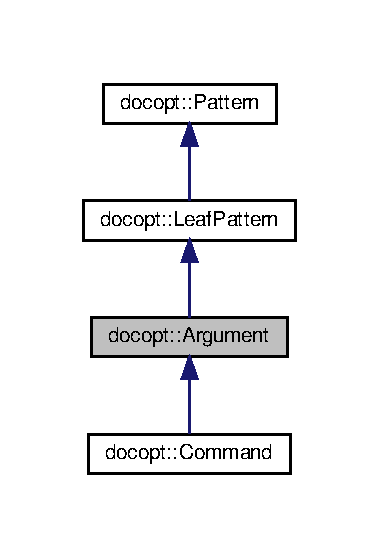
\includegraphics[width=182pt]{classdocopt_1_1Argument__inherit__graph}
\end{center}
\end{figure}


Collaboration diagram for docopt\+:\+:Argument\+:
\nopagebreak
\begin{figure}[H]
\begin{center}
\leavevmode
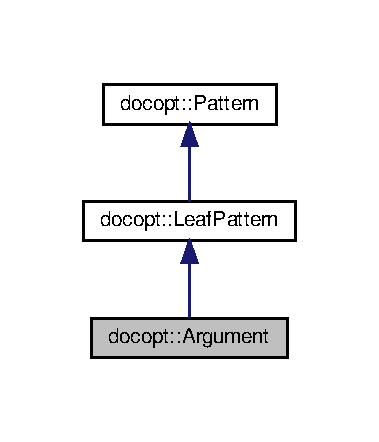
\includegraphics[width=182pt]{classdocopt_1_1Argument__coll__graph}
\end{center}
\end{figure}
\subsection*{Protected Member Functions}
\begin{DoxyCompactItemize}
\item 
\mbox{\Hypertarget{classdocopt_1_1Argument_ab5ebe9ed80895111207a63feeca50f6f}\label{classdocopt_1_1Argument_ab5ebe9ed80895111207a63feeca50f6f}} 
virtual std\+::pair$<$ size\+\_\+t, std\+::shared\+\_\+ptr$<$ \hyperlink{classdocopt_1_1LeafPattern}{Leaf\+Pattern} $>$ $>$ {\bfseries single\+\_\+match} (Pattern\+List const \&left) const override
\end{DoxyCompactItemize}
\subsection*{Additional Inherited Members}


The documentation for this class was generated from the following file\+:\begin{DoxyCompactItemize}
\item 
src/docopt\+\_\+cpp/docopt\+\_\+private.\+h\end{DoxyCompactItemize}

\hypertarget{classupc_1_1array}{}\section{upc\+:\+:array$<$ \+\_\+\+Ty $>$ Class Template Reference}
\label{classupc_1_1array}\index{upc\+::array$<$ \+\_\+\+Ty $>$@{upc\+::array$<$ \+\_\+\+Ty $>$}}


Inheritance diagram for upc\+:\+:array$<$ \+\_\+\+Ty $>$\+:
% FIG 0


Collaboration diagram for upc\+:\+:array$<$ \+\_\+\+Ty $>$\+:
% FIG 1
\subsection*{Public Types}
\begin{DoxyCompactItemize}
\item 
\mbox{\Hypertarget{classupc_1_1array_a9c800a9bf971fc1d7c02a34803f87115}\label{classupc_1_1array_a9c800a9bf971fc1d7c02a34803f87115}} 
typedef \hyperlink{classupc_1_1array}{array}$<$ \+\_\+\+Ty $>$ {\bfseries \+\_\+\+Myt}
\item 
\mbox{\Hypertarget{classupc_1_1array_a85501f086a20ed6686ef78a242b2f302}\label{classupc_1_1array_a85501f086a20ed6686ef78a242b2f302}} 
typedef uint32\+\_\+t {\bfseries size\+\_\+type}
\item 
\mbox{\Hypertarget{classupc_1_1array_a4ef66945898a2c393cff5be41de077d2}\label{classupc_1_1array_a4ef66945898a2c393cff5be41de077d2}} 
typedef \+\_\+\+A\+::pointer {\bfseries \+\_\+\+Tptr}
\item 
\mbox{\Hypertarget{classupc_1_1array_a420718228a4d845721303a19755f0d42}\label{classupc_1_1array_a420718228a4d845721303a19755f0d42}} 
typedef \+\_\+\+A\+::const\+\_\+pointer {\bfseries \+\_\+\+Ctptr}
\item 
\mbox{\Hypertarget{classupc_1_1array_a99066373537d57ee780ce4d3396314f8}\label{classupc_1_1array_a99066373537d57ee780ce4d3396314f8}} 
typedef \+\_\+\+A\+::reference {\bfseries reference}
\item 
\mbox{\Hypertarget{classupc_1_1array_a3b639eaadbf9a2c410d7c02d3d1c01e4}\label{classupc_1_1array_a3b639eaadbf9a2c410d7c02d3d1c01e4}} 
typedef \+\_\+\+A\+::const\+\_\+reference {\bfseries const\+\_\+reference}
\end{DoxyCompactItemize}
\subsection*{Public Member Functions}
\begin{DoxyCompactItemize}
\item 
\mbox{\Hypertarget{classupc_1_1array_a91a96a5d4ba2076aa8d221916d8376a2}\label{classupc_1_1array_a91a96a5d4ba2076aa8d221916d8376a2}} 
{\bfseries array} (unsigned int size=0)
\item 
\mbox{\Hypertarget{classupc_1_1array_a80705655cd83dd14ad6dc38f6711f139}\label{classupc_1_1array_a80705655cd83dd14ad6dc38f6711f139}} 
\+\_\+\+Ctptr {\bfseries v} () const
\item 
\mbox{\Hypertarget{classupc_1_1array_a1b5e50b24d426dd6652139190c0d5b62}\label{classupc_1_1array_a1b5e50b24d426dd6652139190c0d5b62}} 
\+\_\+\+Tptr {\bfseries v} ()
\item 
\mbox{\Hypertarget{classupc_1_1array_aeb72a62336fc9474afdf3fa6f5cea9ca}\label{classupc_1_1array_aeb72a62336fc9474afdf3fa6f5cea9ca}} 
void {\bfseries reset} ()
\end{DoxyCompactItemize}


The documentation for this class was generated from the following file\+:\begin{DoxyCompactItemize}
\item 
src/include/matrix.\+h\end{DoxyCompactItemize}

\hypertarget{classdocopt_1_1BranchPattern}{}\section{docopt\+:\+:Branch\+Pattern Class Reference}
\label{classdocopt_1_1BranchPattern}\index{docopt\+::\+Branch\+Pattern@{docopt\+::\+Branch\+Pattern}}


Inheritance diagram for docopt\+:\+:Branch\+Pattern\+:
% FIG 0


Collaboration diagram for docopt\+:\+:Branch\+Pattern\+:
% FIG 1
\subsection*{Public Member Functions}
\begin{DoxyCompactItemize}
\item 
\mbox{\Hypertarget{classdocopt_1_1BranchPattern_a8a56cbf0c6b730c509cf3922acba2f31}\label{classdocopt_1_1BranchPattern_a8a56cbf0c6b730c509cf3922acba2f31}} 
{\bfseries Branch\+Pattern} (Pattern\+List children=\{\})
\item 
\mbox{\Hypertarget{classdocopt_1_1BranchPattern_ab0c5769d242d5b41c5766ba6d772a34e}\label{classdocopt_1_1BranchPattern_ab0c5769d242d5b41c5766ba6d772a34e}} 
\hyperlink{classdocopt_1_1Pattern}{Pattern} \& {\bfseries fix} ()
\item 
\mbox{\Hypertarget{classdocopt_1_1BranchPattern_abe21ea9bf1f491c64842921bc61d5cdd}\label{classdocopt_1_1BranchPattern_abe21ea9bf1f491c64842921bc61d5cdd}} 
virtual std\+::string const  \& {\bfseries name} () const override
\item 
\mbox{\Hypertarget{classdocopt_1_1BranchPattern_a73fb256384426f7cdad70fcaf13a5195}\label{classdocopt_1_1BranchPattern_a73fb256384426f7cdad70fcaf13a5195}} 
virtual \hyperlink{structdocopt_1_1value}{value} const  \& {\bfseries get\+Value} () const
\item 
\mbox{\Hypertarget{classdocopt_1_1BranchPattern_a7927fbc8ea5f3571f6b2e0e941f3b9b4}\label{classdocopt_1_1BranchPattern_a7927fbc8ea5f3571f6b2e0e941f3b9b4}} 
virtual std\+::vector$<$ \hyperlink{classdocopt_1_1Pattern}{Pattern} $\ast$ $>$ {\bfseries flat} (bool($\ast$filter)(\hyperlink{classdocopt_1_1Pattern}{Pattern} const $\ast$)) override
\item 
\mbox{\Hypertarget{classdocopt_1_1BranchPattern_a48bfc54d124536d84aca67bee7745c34}\label{classdocopt_1_1BranchPattern_a48bfc54d124536d84aca67bee7745c34}} 
virtual void {\bfseries collect\+\_\+leaves} (std\+::vector$<$ \hyperlink{classdocopt_1_1LeafPattern}{Leaf\+Pattern} $\ast$$>$ \&lst) override final
\item 
\mbox{\Hypertarget{classdocopt_1_1BranchPattern_a1b4609af47df9ebba57067e2cb5d762d}\label{classdocopt_1_1BranchPattern_a1b4609af47df9ebba57067e2cb5d762d}} 
void {\bfseries set\+Children} (Pattern\+List children)
\item 
\mbox{\Hypertarget{classdocopt_1_1BranchPattern_aa9bb7831bd3335c84de284086fa89d55}\label{classdocopt_1_1BranchPattern_aa9bb7831bd3335c84de284086fa89d55}} 
Pattern\+List const  \& {\bfseries children} () const
\item 
\mbox{\Hypertarget{classdocopt_1_1BranchPattern_a46f26e4a11c66913472100a2abdb6463}\label{classdocopt_1_1BranchPattern_a46f26e4a11c66913472100a2abdb6463}} 
virtual void {\bfseries fix\+\_\+identities} (Unique\+Pattern\+Set \&patterns)
\item 
\mbox{\Hypertarget{classdocopt_1_1BranchPattern_a0eb838adc74441c109e38c7a07da2519}\label{classdocopt_1_1BranchPattern_a0eb838adc74441c109e38c7a07da2519}} 
virtual size\+\_\+t {\bfseries hash} () const override
\end{DoxyCompactItemize}
\subsection*{Protected Attributes}
\begin{DoxyCompactItemize}
\item 
\mbox{\Hypertarget{classdocopt_1_1BranchPattern_ad34855b839d62d4bfcdfb9cf0b5903cc}\label{classdocopt_1_1BranchPattern_ad34855b839d62d4bfcdfb9cf0b5903cc}} 
Pattern\+List {\bfseries f\+Children}
\end{DoxyCompactItemize}


The documentation for this class was generated from the following file\+:\begin{DoxyCompactItemize}
\item 
src/docopt\+\_\+cpp/docopt\+\_\+private.\+h\end{DoxyCompactItemize}

\hypertarget{classupc_1_1CircularIndex}{}\section{upc\+:\+:Circular\+Index Class Reference}
\label{classupc_1_1CircularIndex}\index{upc\+::\+Circular\+Index@{upc\+::\+Circular\+Index}}


Circular Index used to go through state circular buffer (u)  




{\ttfamily \#include $<$digital\+\_\+filter.\+h$>$}

\subsection*{Public Member Functions}
\begin{DoxyCompactItemize}
\item 
\hyperlink{classupc_1_1CircularIndex_a80c03ec94380d80132ca01b39ef9b0e7}{Circular\+Index} (int s=1)
\begin{DoxyCompactList}\small\item\em buffer size; index goes from 0 ... size-\/1 \end{DoxyCompactList}\item 
\mbox{\Hypertarget{classupc_1_1CircularIndex_abca2976e157594a74d4aa1c06b0c4c2e}\label{classupc_1_1CircularIndex_abca2976e157594a74d4aa1c06b0c4c2e}} 
\hyperlink{classupc_1_1CircularIndex_abca2976e157594a74d4aa1c06b0c4c2e}{Circular\+Index} (\hyperlink{classupc_1_1CircularIndex}{Circular\+Index} \&ci)
\begin{DoxyCompactList}\small\item\em constructor defining size based on other \hyperlink{classupc_1_1CircularIndex}{Circular\+Index} \end{DoxyCompactList}\item 
\mbox{\Hypertarget{classupc_1_1CircularIndex_aa8bfc28723ab87c1ab66262843aac2a5}\label{classupc_1_1CircularIndex_aa8bfc28723ab87c1ab66262843aac2a5}} 
void \hyperlink{classupc_1_1CircularIndex_aa8bfc28723ab87c1ab66262843aac2a5}{resize} (int s)
\begin{DoxyCompactList}\small\item\em Set size of circular index. \end{DoxyCompactList}\item 
\mbox{\Hypertarget{classupc_1_1CircularIndex_a8c02bb1020495ad418f1c0770a03a9f6}\label{classupc_1_1CircularIndex_a8c02bb1020495ad418f1c0770a03a9f6}} 
\hyperlink{classupc_1_1CircularIndex}{Circular\+Index} \& \hyperlink{classupc_1_1CircularIndex_a8c02bb1020495ad418f1c0770a03a9f6}{operator++} ()
\begin{DoxyCompactList}\small\item\em Increment. \end{DoxyCompactList}\item 
\mbox{\Hypertarget{classupc_1_1CircularIndex_a687ae675e4a3f8a95fc69eb0b961c0a5}\label{classupc_1_1CircularIndex_a687ae675e4a3f8a95fc69eb0b961c0a5}} 
\hyperlink{classupc_1_1CircularIndex}{Circular\+Index} \& \hyperlink{classupc_1_1CircularIndex_a687ae675e4a3f8a95fc69eb0b961c0a5}{operator+=} (int i)
\begin{DoxyCompactList}\small\item\em Increment \textquotesingle{}i\textquotesingle{} positions. \end{DoxyCompactList}\item 
\mbox{\Hypertarget{classupc_1_1CircularIndex_a1e03db5aad51600b2804b7866af81b01}\label{classupc_1_1CircularIndex_a1e03db5aad51600b2804b7866af81b01}} 
\hyperlink{classupc_1_1CircularIndex}{Circular\+Index} \& \hyperlink{classupc_1_1CircularIndex_a1e03db5aad51600b2804b7866af81b01}{operator+} (int i)
\begin{DoxyCompactList}\small\item\em Increment \textquotesingle{}i\textquotesingle{} positions. \end{DoxyCompactList}\item 
\mbox{\Hypertarget{classupc_1_1CircularIndex_a4527e57789e25c6157111ab491cc38a9}\label{classupc_1_1CircularIndex_a4527e57789e25c6157111ab491cc38a9}} 
\hyperlink{classupc_1_1CircularIndex}{Circular\+Index} \& \hyperlink{classupc_1_1CircularIndex_a4527e57789e25c6157111ab491cc38a9}{operator-\/-\/} ()
\begin{DoxyCompactList}\small\item\em Decrement. \end{DoxyCompactList}\item 
\mbox{\Hypertarget{classupc_1_1CircularIndex_a4b2892d8a0b891b90bcb34ee55c3d613}\label{classupc_1_1CircularIndex_a4b2892d8a0b891b90bcb34ee55c3d613}} 
\hyperlink{classupc_1_1CircularIndex}{Circular\+Index} \& \hyperlink{classupc_1_1CircularIndex_a4b2892d8a0b891b90bcb34ee55c3d613}{operator-\/=} (int i)
\begin{DoxyCompactList}\small\item\em Decrement \textquotesingle{}i\textquotesingle{} positions. \end{DoxyCompactList}\item 
\mbox{\Hypertarget{classupc_1_1CircularIndex_a7745755030622a01389f2133632d7f76}\label{classupc_1_1CircularIndex_a7745755030622a01389f2133632d7f76}} 
\hyperlink{classupc_1_1CircularIndex}{Circular\+Index} \& \hyperlink{classupc_1_1CircularIndex_a7745755030622a01389f2133632d7f76}{operator-\/} (int i)
\begin{DoxyCompactList}\small\item\em Decrement \textquotesingle{}i\textquotesingle{} positions. \end{DoxyCompactList}\item 
\mbox{\Hypertarget{classupc_1_1CircularIndex_ab0961d598cc0a51a2990e8823f71a332}\label{classupc_1_1CircularIndex_ab0961d598cc0a51a2990e8823f71a332}} 
{\bfseries operator int} ()
\item 
\mbox{\Hypertarget{classupc_1_1CircularIndex_ab23f2d6ba2b5781153bcf6383cce8afc}\label{classupc_1_1CircularIndex_ab23f2d6ba2b5781153bcf6383cce8afc}} 
\hyperlink{classupc_1_1CircularIndex}{Circular\+Index} \& \hyperlink{classupc_1_1CircularIndex_ab23f2d6ba2b5781153bcf6383cce8afc}{operator=} (const \hyperlink{classupc_1_1CircularIndex}{Circular\+Index} \&ci)
\begin{DoxyCompactList}\small\item\em !\+Casting from \hyperlink{classupc_1_1CircularIndex}{Circular\+Index} to int, returning int. \end{DoxyCompactList}\end{DoxyCompactItemize}


\subsection{Detailed Description}
Circular Index used to go through state circular buffer (u) 

The circular index is a simple class to address a circular buffer. Once the buffer size is defined, you can add or substract and the index remains inside the buffer. A casting operator to int is provided.

Example\+: 
\begin{DoxyCode}
\textcolor{keywordtype}{float} x[8]=\{0,1,2,4,5,6,7\};
\hyperlink{classupc_1_1CircularIndex_a80c03ec94380d80132ca01b39ef9b0e7}{CircularIndex} ci(8);
\textcolor{keywordtype}{int} n=10; \textcolor{keywordtype}{float} z=0.0F;
\textcolor{keywordflow}{for} (n=0; n< 10; ++n, ++ci)
    z += x[ci+1] - x[ci-1];
\end{DoxyCode}
 Operations +, +=, ++, -\/, -\/=, -- are defined 

\subsection{Constructor \& Destructor Documentation}
\mbox{\Hypertarget{classupc_1_1CircularIndex_a80c03ec94380d80132ca01b39ef9b0e7}\label{classupc_1_1CircularIndex_a80c03ec94380d80132ca01b39ef9b0e7}} 
\index{upc\+::\+Circular\+Index@{upc\+::\+Circular\+Index}!Circular\+Index@{Circular\+Index}}
\index{Circular\+Index@{Circular\+Index}!upc\+::\+Circular\+Index@{upc\+::\+Circular\+Index}}
\subsubsection{\texorpdfstring{Circular\+Index()}{CircularIndex()}}
{\footnotesize\ttfamily upc\+::\+Circular\+Index\+::\+Circular\+Index (\begin{DoxyParamCaption}\item[{int}]{s = {\ttfamily 1} }\end{DoxyParamCaption})\hspace{0.3cm}{\ttfamily [inline]}}



buffer size; index goes from 0 ... size-\/1 

default\+: size=1; not very useful (index can only be 0) 

The documentation for this class was generated from the following file\+:\begin{DoxyCompactItemize}
\item 
src/include/digital\+\_\+filter.\+h\end{DoxyCompactItemize}

\hypertarget{classdocopt_1_1Command}{}\section{docopt\+:\+:Command Class Reference}
\label{classdocopt_1_1Command}\index{docopt\+::\+Command@{docopt\+::\+Command}}


Inheritance diagram for docopt\+:\+:Command\+:
% FIG 0


Collaboration diagram for docopt\+:\+:Command\+:
% FIG 1
\subsection*{Public Member Functions}
\begin{DoxyCompactItemize}
\item 
\mbox{\Hypertarget{classdocopt_1_1Command_a94e1480a83f75acf6c1e7d506253c319}\label{classdocopt_1_1Command_a94e1480a83f75acf6c1e7d506253c319}} 
{\bfseries Command} (std\+::string name, \hyperlink{structdocopt_1_1value}{value} v=\hyperlink{structdocopt_1_1value}{value}\{false\})
\end{DoxyCompactItemize}
\subsection*{Protected Member Functions}
\begin{DoxyCompactItemize}
\item 
\mbox{\Hypertarget{classdocopt_1_1Command_a914bd0c3225c4e14ed55bacb873ca87f}\label{classdocopt_1_1Command_a914bd0c3225c4e14ed55bacb873ca87f}} 
virtual std\+::pair$<$ size\+\_\+t, std\+::shared\+\_\+ptr$<$ \hyperlink{classdocopt_1_1LeafPattern}{Leaf\+Pattern} $>$ $>$ {\bfseries single\+\_\+match} (Pattern\+List const \&left) const override
\end{DoxyCompactItemize}


The documentation for this class was generated from the following file\+:\begin{DoxyCompactItemize}
\item 
src/docopt\+\_\+cpp/docopt\+\_\+private.\+h\end{DoxyCompactItemize}

\hypertarget{classupc_1_1DigitalFilter}{}\section{upc\+:\+:Digital\+Filter Class Reference}
\label{classupc_1_1DigitalFilter}\index{upc\+::\+Digital\+Filter@{upc\+::\+Digital\+Filter}}


Digital filter implemented using direct form.  




{\ttfamily \#include $<$digital\+\_\+filter.\+h$>$}

\subsection*{Public Member Functions}
\begin{DoxyCompactItemize}
\item 
\mbox{\Hypertarget{classupc_1_1DigitalFilter_a3d8e61b92170380d06b26aee1ebc1f16}\label{classupc_1_1DigitalFilter_a3d8e61b92170380d06b26aee1ebc1f16}} 
\hyperlink{classupc_1_1DigitalFilter_a3d8e61b92170380d06b26aee1ebc1f16}{Digital\+Filter} (const std\+::vector$<$ float $>$ \&\+\_\+a, const std\+::vector$<$ float $>$ \&\+\_\+b, float g=1.\+0\+F)
\begin{DoxyCompactList}\small\item\em Create filter. \end{DoxyCompactList}\item 
\mbox{\Hypertarget{classupc_1_1DigitalFilter_ac3c32e0d51a88354482f13528e9a7842}\label{classupc_1_1DigitalFilter_ac3c32e0d51a88354482f13528e9a7842}} 
\hyperlink{classupc_1_1DigitalFilter_ac3c32e0d51a88354482f13528e9a7842}{Digital\+Filter} ()
\begin{DoxyCompactList}\small\item\em create void filter H(z) = 1 \end{DoxyCompactList}\item 
\mbox{\Hypertarget{classupc_1_1DigitalFilter_ade3c3a24bbfbc1b2edbf4bcd0885a9e6}\label{classupc_1_1DigitalFilter_ade3c3a24bbfbc1b2edbf4bcd0885a9e6}} 
void \hyperlink{classupc_1_1DigitalFilter_ade3c3a24bbfbc1b2edbf4bcd0885a9e6}{set\+\_\+a} (std\+::vector$<$ float $>$ const \&A)
\begin{DoxyCompactList}\small\item\em Change denominator (state conditions only cleaned if order changes) \end{DoxyCompactList}\item 
\mbox{\Hypertarget{classupc_1_1DigitalFilter_a9f23a5e9db027eb0c9b70bd9b5d08e09}\label{classupc_1_1DigitalFilter_a9f23a5e9db027eb0c9b70bd9b5d08e09}} 
void \hyperlink{classupc_1_1DigitalFilter_a9f23a5e9db027eb0c9b70bd9b5d08e09}{set\+\_\+b} (const std\+::vector$<$ float $>$ \&B)
\begin{DoxyCompactList}\small\item\em Change denominator (state conditions only cleaned if order changes) \end{DoxyCompactList}\item 
\hyperlink{classupc_1_1DigitalFilter_a54937beb73f0789cb9265498522da628}{Digital\+Filter} (const \hyperlink{classupc_1_1DigitalFilter}{Digital\+Filter} \&f)
\item 
\mbox{\Hypertarget{classupc_1_1DigitalFilter_a26527559b1b71aad240deca22f5599ec}\label{classupc_1_1DigitalFilter_a26527559b1b71aad240deca22f5599ec}} 
\hyperlink{classupc_1_1DigitalFilter}{Digital\+Filter} \& \hyperlink{classupc_1_1DigitalFilter_a26527559b1b71aad240deca22f5599ec}{operator=} (const \hyperlink{classupc_1_1DigitalFilter}{Digital\+Filter} \&f)
\begin{DoxyCompactList}\small\item\em Asign operator (copy a filter from other) \end{DoxyCompactList}\item 
\mbox{\Hypertarget{classupc_1_1DigitalFilter_a2b97aaeacac8b5a8b52e1bd8fc295970}\label{classupc_1_1DigitalFilter_a2b97aaeacac8b5a8b52e1bd8fc295970}} 
void \hyperlink{classupc_1_1DigitalFilter_a2b97aaeacac8b5a8b52e1bd8fc295970}{set\+\_\+resonator} (float norm\+\_\+central\+\_\+freq, float norm\+\_\+bandwidth)
\begin{DoxyCompactList}\small\item\em Second order AR band-\/pass filter defined by central frequency and bandwidth. \end{DoxyCompactList}\item 
\mbox{\Hypertarget{classupc_1_1DigitalFilter_a506905346c44ac46c292ea1fa1212c3e}\label{classupc_1_1DigitalFilter_a506905346c44ac46c292ea1fa1212c3e}} 
void {\bfseries set\+\_\+gain} (float g)
\item 
\mbox{\Hypertarget{classupc_1_1DigitalFilter_ad6c0f9584687642434081448f85d89f9}\label{classupc_1_1DigitalFilter_ad6c0f9584687642434081448f85d89f9}} 
void \hyperlink{classupc_1_1DigitalFilter_ad6c0f9584687642434081448f85d89f9}{clear} ()
\begin{DoxyCompactList}\small\item\em clean state conditions \end{DoxyCompactList}\item 
\mbox{\Hypertarget{classupc_1_1DigitalFilter_a8d8f578b514a2dd58a545a68fdf441ee}\label{classupc_1_1DigitalFilter_a8d8f578b514a2dd58a545a68fdf441ee}} 
float \hyperlink{classupc_1_1DigitalFilter_a8d8f578b514a2dd58a545a68fdf441ee}{operator()} (float x)
\begin{DoxyCompactList}\small\item\em Filter one sample. \end{DoxyCompactList}\item 
\mbox{\Hypertarget{classupc_1_1DigitalFilter_aea8cdd6504cf9c4ae1a6d9a28e1bcaa4}\label{classupc_1_1DigitalFilter_aea8cdd6504cf9c4ae1a6d9a28e1bcaa4}} 
std\+::vector$<$ float $>$ \hyperlink{classupc_1_1DigitalFilter_aea8cdd6504cf9c4ae1a6d9a28e1bcaa4}{operator()} (const std\+::vector$<$ float $>$ \&x)
\begin{DoxyCompactList}\small\item\em Filter a vector of samples. \end{DoxyCompactList}\item 
\mbox{\Hypertarget{classupc_1_1DigitalFilter_a08b53e2a3884053f4a48d6860194cccb}\label{classupc_1_1DigitalFilter_a08b53e2a3884053f4a48d6860194cccb}} 
void \hyperlink{classupc_1_1DigitalFilter_a08b53e2a3884053f4a48d6860194cccb}{operator()} (std\+::vector$<$ float $>$\+::const\+\_\+iterator beg\+Src, std\+::vector$<$ float $>$\+::const\+\_\+iterator end\+Src, std\+::vector$<$ float $>$\+::iterator beg\+Dst)
\begin{DoxyCompactList}\small\item\em Filter several samples, from beg\+Src to end\+Src, and save at beg\+Dst and following positions. \end{DoxyCompactList}\item 
std\+::vector$<$ float $>$ \hyperlink{classupc_1_1DigitalFilter_a03537f0f0604b772f8f6ee3cc08f194e}{freqz} (std\+::vector$<$ float $>$ const freq, bool db=true) const
\item 
std\+::vector$<$ float $>$ \hyperlink{classupc_1_1DigitalFilter_aaccd48246b8f0154725d40d43ae52268}{freqz} (unsigned int N, bool db=true) const
\item 
float \hyperlink{classupc_1_1DigitalFilter_aee8d8470871b79ff465459ad0bedd833}{sfreqz} (float freq, bool db=true) const
\end{DoxyCompactItemize}


\subsection{Detailed Description}
Digital filter implemented using direct form. 

This class implements digital filtering. The filter is stored as rational funcion H(z) = g B(z)/A(z) Being g\+: gain B(z) = b0 +b1 z$^\wedge$-\/1 + b2 z$^\wedge$-\/2 ... bm z$^\wedge$-\/m A(z) = a0 +a1 z$^\wedge$-\/1 + a2 z$^\wedge$-\/2 ... an z$^\wedge$-\/n

The state conditions are saved after each call to the filter. The filter is implemented using the direct form. Y(z) = B(z)/A(z) X(z) =$>$ U(z) = X(z)/A(z); Y(z) = B(z) U(z) State conditions\+: u\mbox{[}n\mbox{]}

The state conditions are only cleared either\+:
\begin{DoxyItemize}
\item explicitely calling clean()
\item by a change in filter coeficients that imply an order filter
\end{DoxyItemize}

The filters coefficients are set using \hyperlink{classupc_1_1DigitalFilter_ade3c3a24bbfbc1b2edbf4bcd0885a9e6}{set\+\_\+a()}, \hyperlink{classupc_1_1DigitalFilter_a9f23a5e9db027eb0c9b70bd9b5d08e09}{set\+\_\+b()}, set\+\_\+gain(). An alternative convinient method exist for 2nd order resonators, using the central frequency and the resonator bandwidth\+: \hyperlink{classupc_1_1DigitalFilter_a2b97aaeacac8b5a8b52e1bd8fc295970}{set\+\_\+resonator()} 

\subsection{Constructor \& Destructor Documentation}
\mbox{\Hypertarget{classupc_1_1DigitalFilter_a54937beb73f0789cb9265498522da628}\label{classupc_1_1DigitalFilter_a54937beb73f0789cb9265498522da628}} 
\index{upc\+::\+Digital\+Filter@{upc\+::\+Digital\+Filter}!Digital\+Filter@{Digital\+Filter}}
\index{Digital\+Filter@{Digital\+Filter}!upc\+::\+Digital\+Filter@{upc\+::\+Digital\+Filter}}
\subsubsection{\texorpdfstring{Digital\+Filter()}{DigitalFilter()}}
{\footnotesize\ttfamily upc\+::\+Digital\+Filter\+::\+Digital\+Filter (\begin{DoxyParamCaption}\item[{const \hyperlink{classupc_1_1DigitalFilter}{Digital\+Filter} \&}]{f }\end{DoxyParamCaption})\hspace{0.3cm}{\ttfamily [inline]}}

Create filter 

\subsection{Member Function Documentation}
\mbox{\Hypertarget{classupc_1_1DigitalFilter_a03537f0f0604b772f8f6ee3cc08f194e}\label{classupc_1_1DigitalFilter_a03537f0f0604b772f8f6ee3cc08f194e}} 
\index{upc\+::\+Digital\+Filter@{upc\+::\+Digital\+Filter}!freqz@{freqz}}
\index{freqz@{freqz}!upc\+::\+Digital\+Filter@{upc\+::\+Digital\+Filter}}
\subsubsection{\texorpdfstring{freqz()}{freqz()}\hspace{0.1cm}{\footnotesize\ttfamily [1/2]}}
{\footnotesize\ttfamily std\+::vector$<$ float $>$ upc\+::\+Digital\+Filter\+::freqz (\begin{DoxyParamCaption}\item[{std\+::vector$<$ float $>$ const}]{freq,  }\item[{bool}]{db = {\ttfamily true} }\end{DoxyParamCaption}) const}

Get freq. response of filter in the given frequencies (freq). \hyperlink{classupc_1_1DigitalFilter_aee8d8470871b79ff465459ad0bedd833}{sfreqz()} is called for each given frequency \mbox{\Hypertarget{classupc_1_1DigitalFilter_aaccd48246b8f0154725d40d43ae52268}\label{classupc_1_1DigitalFilter_aaccd48246b8f0154725d40d43ae52268}} 
\index{upc\+::\+Digital\+Filter@{upc\+::\+Digital\+Filter}!freqz@{freqz}}
\index{freqz@{freqz}!upc\+::\+Digital\+Filter@{upc\+::\+Digital\+Filter}}
\subsubsection{\texorpdfstring{freqz()}{freqz()}\hspace{0.1cm}{\footnotesize\ttfamily [2/2]}}
{\footnotesize\ttfamily std\+::vector$<$ float $>$ upc\+::\+Digital\+Filter\+::freqz (\begin{DoxyParamCaption}\item[{unsigned int}]{N,  }\item[{bool}]{db = {\ttfamily true} }\end{DoxyParamCaption}) const}

Get freq. response of filter in N discrite frequencies, from 0 to 0.\+5. \hyperlink{classupc_1_1DigitalFilter_aee8d8470871b79ff465459ad0bedd833}{sfreqz()} is called for each given frequency \mbox{\Hypertarget{classupc_1_1DigitalFilter_aee8d8470871b79ff465459ad0bedd833}\label{classupc_1_1DigitalFilter_aee8d8470871b79ff465459ad0bedd833}} 
\index{upc\+::\+Digital\+Filter@{upc\+::\+Digital\+Filter}!sfreqz@{sfreqz}}
\index{sfreqz@{sfreqz}!upc\+::\+Digital\+Filter@{upc\+::\+Digital\+Filter}}
\subsubsection{\texorpdfstring{sfreqz()}{sfreqz()}}
{\footnotesize\ttfamily float upc\+::\+Digital\+Filter\+::sfreqz (\begin{DoxyParamCaption}\item[{float}]{freq,  }\item[{bool}]{db = {\ttfamily true} }\end{DoxyParamCaption}) const}

Get freq. response of filter in the given frequency (freq). freq is the digital frequency, f/fsampling, with range in \mbox{[}0,0.\+5\mbox{]} If db is true, provide the result in dB\+: 20log($\vert$H(e$^\wedge$j2pif)$\vert$; Otherwise, the results is the squared module, $\vert$\+H$\vert$$^\wedge$2 

The documentation for this class was generated from the following files\+:\begin{DoxyCompactItemize}
\item 
src/include/digital\+\_\+filter.\+h\item 
src/pav/digital\+\_\+filter.\+cpp\end{DoxyCompactItemize}

\hypertarget{classupc_1_1Directory}{}\section{upc\+:\+:Directory Class Reference}
\label{classupc_1_1Directory}\index{upc\+::\+Directory@{upc\+::\+Directory}}


Inheritance diagram for upc\+:\+:Directory\+:
\nopagebreak
\begin{figure}[H]
\begin{center}
\leavevmode
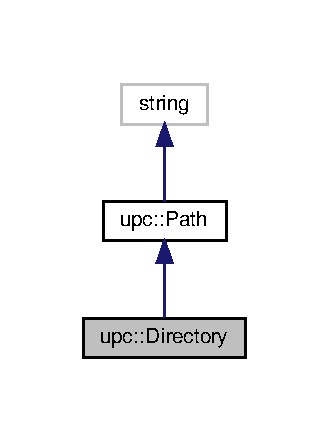
\includegraphics[width=158pt]{classupc_1_1Directory__inherit__graph}
\end{center}
\end{figure}


Collaboration diagram for upc\+:\+:Directory\+:
\nopagebreak
\begin{figure}[H]
\begin{center}
\leavevmode
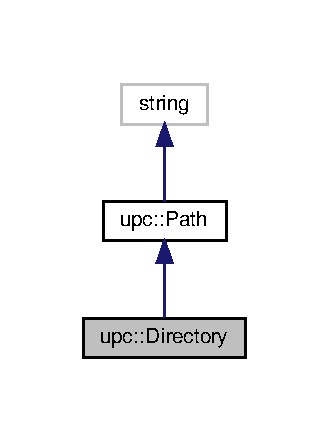
\includegraphics[width=158pt]{classupc_1_1Directory__coll__graph}
\end{center}
\end{figure}
\subsection*{Public Member Functions}
\begin{DoxyCompactItemize}
\item 
\mbox{\Hypertarget{classupc_1_1Directory_a4b6321fb7644d3dcf225e2e666b837da}\label{classupc_1_1Directory_a4b6321fb7644d3dcf225e2e666b837da}} 
{\bfseries Directory} (const \hyperlink{classupc_1_1Path}{Path} \&p)
\item 
\mbox{\Hypertarget{classupc_1_1Directory_aca9acc226940f166429185989023727f}\label{classupc_1_1Directory_aca9acc226940f166429185989023727f}} 
{\bfseries Directory} (const string \&p)
\item 
\mbox{\Hypertarget{classupc_1_1Directory_afb8c8e0bc50664d8505e0fa392f99657}\label{classupc_1_1Directory_afb8c8e0bc50664d8505e0fa392f99657}} 
{\bfseries Directory} (const char $\ast$p)
\item 
\mbox{\Hypertarget{classupc_1_1Directory_ac1ea823e51c240b8f90e6057f2694bd5}\label{classupc_1_1Directory_ac1ea823e51c240b8f90e6057f2694bd5}} 
bool {\bfseries make} () const
\item 
\mbox{\Hypertarget{classupc_1_1Directory_a110a8b694850028b67a30167fd8bc575}\label{classupc_1_1Directory_a110a8b694850028b67a30167fd8bc575}} 
bool {\bfseries exist} () const
\end{DoxyCompactItemize}


The documentation for this class was generated from the following files\+:\begin{DoxyCompactItemize}
\item 
src/include/filename.\+h\item 
src/pav/filename.\+cpp\end{DoxyCompactItemize}

\hypertarget{structdocopt_1_1DocoptArgumentError}{}\section{docopt\+:\+:Docopt\+Argument\+Error Struct Reference}
\label{structdocopt_1_1DocoptArgumentError}\index{docopt\+::\+Docopt\+Argument\+Error@{docopt\+::\+Docopt\+Argument\+Error}}


Inheritance diagram for docopt\+:\+:Docopt\+Argument\+Error\+:
\nopagebreak
\begin{figure}[H]
\begin{center}
\leavevmode
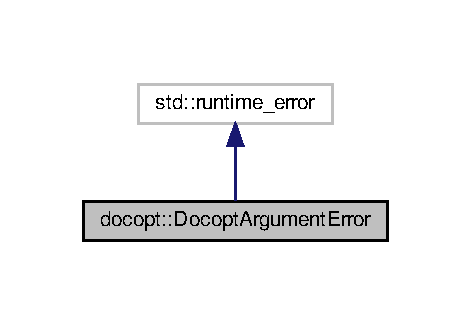
\includegraphics[width=226pt]{structdocopt_1_1DocoptArgumentError__inherit__graph}
\end{center}
\end{figure}


Collaboration diagram for docopt\+:\+:Docopt\+Argument\+Error\+:
\nopagebreak
\begin{figure}[H]
\begin{center}
\leavevmode
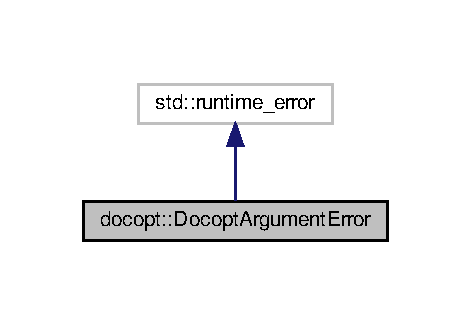
\includegraphics[width=226pt]{structdocopt_1_1DocoptArgumentError__coll__graph}
\end{center}
\end{figure}


The documentation for this struct was generated from the following file\+:\begin{DoxyCompactItemize}
\item 
src/docopt\+\_\+cpp/docopt.\+h\end{DoxyCompactItemize}

\hypertarget{structdocopt_1_1DocoptExitHelp}{}\section{docopt\+:\+:Docopt\+Exit\+Help Struct Reference}
\label{structdocopt_1_1DocoptExitHelp}\index{docopt\+::\+Docopt\+Exit\+Help@{docopt\+::\+Docopt\+Exit\+Help}}


Inheritance diagram for docopt\+:\+:Docopt\+Exit\+Help\+:
\nopagebreak
\begin{figure}[H]
\begin{center}
\leavevmode
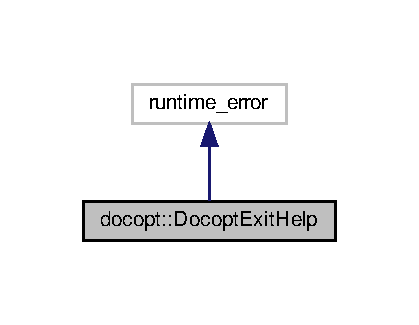
\includegraphics[width=201pt]{structdocopt_1_1DocoptExitHelp__inherit__graph}
\end{center}
\end{figure}


Collaboration diagram for docopt\+:\+:Docopt\+Exit\+Help\+:
\nopagebreak
\begin{figure}[H]
\begin{center}
\leavevmode
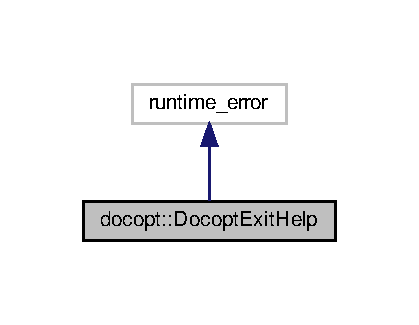
\includegraphics[width=201pt]{structdocopt_1_1DocoptExitHelp__coll__graph}
\end{center}
\end{figure}


The documentation for this struct was generated from the following file\+:\begin{DoxyCompactItemize}
\item 
src/docopt\+\_\+cpp/docopt.\+h\end{DoxyCompactItemize}

\hypertarget{structdocopt_1_1DocoptExitVersion}{}\section{docopt\+:\+:Docopt\+Exit\+Version Struct Reference}
\label{structdocopt_1_1DocoptExitVersion}\index{docopt\+::\+Docopt\+Exit\+Version@{docopt\+::\+Docopt\+Exit\+Version}}


Inheritance diagram for docopt\+:\+:Docopt\+Exit\+Version\+:
% FIG 0


Collaboration diagram for docopt\+:\+:Docopt\+Exit\+Version\+:
% FIG 1


The documentation for this struct was generated from the following file\+:\begin{DoxyCompactItemize}
\item 
src/docopt\+\_\+cpp/docopt.\+h\end{DoxyCompactItemize}

\hypertarget{structdocopt_1_1DocoptLanguageError}{}\section{docopt\+:\+:Docopt\+Language\+Error Struct Reference}
\label{structdocopt_1_1DocoptLanguageError}\index{docopt\+::\+Docopt\+Language\+Error@{docopt\+::\+Docopt\+Language\+Error}}


Inheritance diagram for docopt\+:\+:Docopt\+Language\+Error\+:
% FIG 0


Collaboration diagram for docopt\+:\+:Docopt\+Language\+Error\+:
% FIG 1


The documentation for this struct was generated from the following file\+:\begin{DoxyCompactItemize}
\item 
src/docopt\+\_\+cpp/docopt.\+h\end{DoxyCompactItemize}

\hypertarget{classffft_1_1DynArray}{}\section{ffft\+:\+:Dyn\+Array$<$ T $>$ Class Template Reference}
\label{classffft_1_1DynArray}\index{ffft\+::\+Dyn\+Array$<$ T $>$@{ffft\+::\+Dyn\+Array$<$ T $>$}}
\subsection*{Public Types}
\begin{DoxyCompactItemize}
\item 
\mbox{\Hypertarget{classffft_1_1DynArray_aa21fa88c73e511acb18a7e778190ab02}\label{classffft_1_1DynArray_aa21fa88c73e511acb18a7e778190ab02}} 
typedef T {\bfseries Data\+Type}
\end{DoxyCompactItemize}
\subsection*{Public Member Functions}
\begin{DoxyCompactItemize}
\item 
\mbox{\Hypertarget{classffft_1_1DynArray_a26919351a30b4be36c3e3ee500a7c6a7}\label{classffft_1_1DynArray_a26919351a30b4be36c3e3ee500a7c6a7}} 
{\bfseries Dyn\+Array} (long size)
\item 
\mbox{\Hypertarget{classffft_1_1DynArray_a36eebe95c5f12a370d9f4c281a215c05}\label{classffft_1_1DynArray_a36eebe95c5f12a370d9f4c281a215c05}} 
long {\bfseries size} () const
\item 
\mbox{\Hypertarget{classffft_1_1DynArray_a3879167bca7e35ee75596318f67e2930}\label{classffft_1_1DynArray_a3879167bca7e35ee75596318f67e2930}} 
void {\bfseries resize} (long size)
\item 
\mbox{\Hypertarget{classffft_1_1DynArray_a74ff037cb856b4a62c81147d357697bc}\label{classffft_1_1DynArray_a74ff037cb856b4a62c81147d357697bc}} 
const Data\+Type \& {\bfseries operator\mbox{[}$\,$\mbox{]}} (long pos) const
\item 
\mbox{\Hypertarget{classffft_1_1DynArray_a79c769ea7c52d0fbbe67831380b9a89c}\label{classffft_1_1DynArray_a79c769ea7c52d0fbbe67831380b9a89c}} 
Data\+Type \& {\bfseries operator\mbox{[}$\,$\mbox{]}} (long pos)
\end{DoxyCompactItemize}


The documentation for this class was generated from the following files\+:\begin{DoxyCompactItemize}
\item 
src/include/ffft/Dyn\+Array.\+h\item 
src/include/ffft/Dyn\+Array.\+hpp\end{DoxyCompactItemize}

\hypertarget{classdocopt_1_1Either}{}\section{docopt\+:\+:Either Class Reference}
\label{classdocopt_1_1Either}\index{docopt\+::\+Either@{docopt\+::\+Either}}


Inheritance diagram for docopt\+:\+:Either\+:
\nopagebreak
\begin{figure}[H]
\begin{center}
\leavevmode
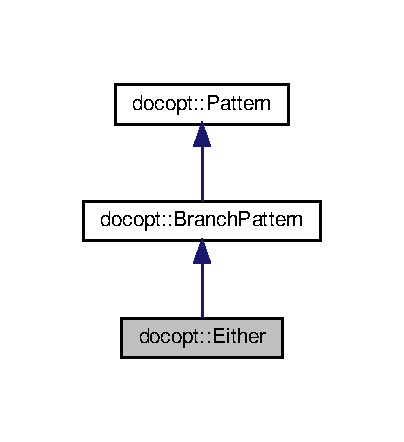
\includegraphics[width=194pt]{classdocopt_1_1Either__inherit__graph}
\end{center}
\end{figure}


Collaboration diagram for docopt\+:\+:Either\+:
\nopagebreak
\begin{figure}[H]
\begin{center}
\leavevmode
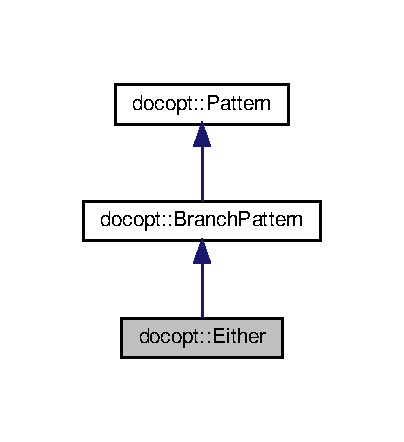
\includegraphics[width=194pt]{classdocopt_1_1Either__coll__graph}
\end{center}
\end{figure}
\subsection*{Public Member Functions}
\begin{DoxyCompactItemize}
\item 
\mbox{\Hypertarget{classdocopt_1_1Either_aedbb09ed31a6c321d274040e3179d449}\label{classdocopt_1_1Either_aedbb09ed31a6c321d274040e3179d449}} 
bool {\bfseries match} (Pattern\+List \&left, std\+::vector$<$ std\+::shared\+\_\+ptr$<$ \hyperlink{classdocopt_1_1LeafPattern}{Leaf\+Pattern} $>$$>$ \&collected) const override
\end{DoxyCompactItemize}
\subsection*{Additional Inherited Members}


The documentation for this class was generated from the following file\+:\begin{DoxyCompactItemize}
\item 
src/docopt\+\_\+cpp/docopt\+\_\+private.\+h\end{DoxyCompactItemize}

\hypertarget{classupc_1_1Ext}{}\section{upc\+:\+:Ext Class Reference}
\label{classupc_1_1Ext}\index{upc\+::\+Ext@{upc\+::\+Ext}}


Inheritance diagram for upc\+:\+:Ext\+:
\nopagebreak
\begin{figure}[H]
\begin{center}
\leavevmode
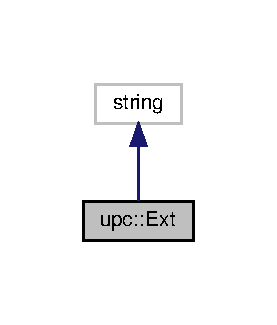
\includegraphics[width=133pt]{classupc_1_1Ext__inherit__graph}
\end{center}
\end{figure}


Collaboration diagram for upc\+:\+:Ext\+:
\nopagebreak
\begin{figure}[H]
\begin{center}
\leavevmode
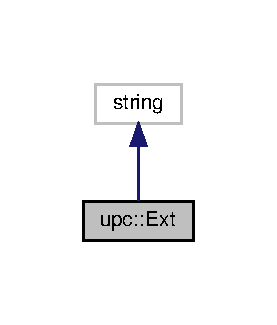
\includegraphics[width=133pt]{classupc_1_1Ext__coll__graph}
\end{center}
\end{figure}
\subsection*{Public Member Functions}
\begin{DoxyCompactItemize}
\item 
\mbox{\Hypertarget{classupc_1_1Ext_af9636b92ecb5e6f5d0f16ae4d968c21a}\label{classupc_1_1Ext_af9636b92ecb5e6f5d0f16ae4d968c21a}} 
{\bfseries Ext} (const string \&str)
\item 
\mbox{\Hypertarget{classupc_1_1Ext_a0e3b4b899d14b0bef3dbf566a38086ae}\label{classupc_1_1Ext_a0e3b4b899d14b0bef3dbf566a38086ae}} 
{\bfseries Ext} (const char $\ast$str)
\end{DoxyCompactItemize}


The documentation for this class was generated from the following file\+:\begin{DoxyCompactItemize}
\item 
src/include/filename.\+h\end{DoxyCompactItemize}

\hypertarget{classffft_1_1FFTReal}{}\section{ffft\+:\+:F\+F\+T\+Real$<$ DT $>$ Class Template Reference}
\label{classffft_1_1FFTReal}\index{ffft\+::\+F\+F\+T\+Real$<$ D\+T $>$@{ffft\+::\+F\+F\+T\+Real$<$ D\+T $>$}}
\subsection*{Public Types}
\begin{DoxyCompactItemize}
\item 
\mbox{\Hypertarget{classffft_1_1FFTReal_a39f5a2ec14c15f9198268500716e5dba}\label{classffft_1_1FFTReal_a39f5a2ec14c15f9198268500716e5dba}} 
enum \{ {\bfseries M\+A\+X\+\_\+\+B\+I\+T\+\_\+\+D\+E\+P\+TH} = 30
 \}
\item 
\mbox{\Hypertarget{classffft_1_1FFTReal_a606148f1cf8c3b7d705473932fc063d1}\label{classffft_1_1FFTReal_a606148f1cf8c3b7d705473932fc063d1}} 
typedef DT {\bfseries Data\+Type}
\end{DoxyCompactItemize}
\subsection*{Public Member Functions}
\begin{DoxyCompactItemize}
\item 
\mbox{\Hypertarget{classffft_1_1FFTReal_a627db4d781235302c3a229fc4d7a10ba}\label{classffft_1_1FFTReal_a627db4d781235302c3a229fc4d7a10ba}} 
{\bfseries F\+F\+T\+Real} (long length)
\item 
\mbox{\Hypertarget{classffft_1_1FFTReal_ac7e604c1ab7d7281d6b17ae1aa86ff36}\label{classffft_1_1FFTReal_ac7e604c1ab7d7281d6b17ae1aa86ff36}} 
long {\bfseries get\+\_\+length} () const
\item 
\mbox{\Hypertarget{classffft_1_1FFTReal_aefe76dd83673ecb01d1216b4c636d1e0}\label{classffft_1_1FFTReal_aefe76dd83673ecb01d1216b4c636d1e0}} 
void {\bfseries do\+\_\+fft} (Data\+Type f \mbox{[}$\,$\mbox{]}, const Data\+Type x \mbox{[}$\,$\mbox{]}) const
\item 
\mbox{\Hypertarget{classffft_1_1FFTReal_aec086bf8d016e8cf9cd7351502c92551}\label{classffft_1_1FFTReal_aec086bf8d016e8cf9cd7351502c92551}} 
void {\bfseries do\+\_\+ifft} (const Data\+Type f \mbox{[}$\,$\mbox{]}, Data\+Type x \mbox{[}$\,$\mbox{]}) const
\item 
\mbox{\Hypertarget{classffft_1_1FFTReal_a80050e7511e3662d121720f56dbd9cd7}\label{classffft_1_1FFTReal_a80050e7511e3662d121720f56dbd9cd7}} 
void {\bfseries rescale} (Data\+Type x \mbox{[}$\,$\mbox{]}) const
\item 
\mbox{\Hypertarget{classffft_1_1FFTReal_ae91999ceb42d32eef5bdd0d16db989d5}\label{classffft_1_1FFTReal_ae91999ceb42d32eef5bdd0d16db989d5}} 
Data\+Type $\ast$ {\bfseries use\+\_\+buffer} () const
\end{DoxyCompactItemize}


The documentation for this class was generated from the following files\+:\begin{DoxyCompactItemize}
\item 
src/include/ffft/F\+F\+T\+Real.\+h\item 
src/include/ffft/F\+F\+T\+Real.\+hpp\end{DoxyCompactItemize}

\hypertarget{classupc_1_1FileInfo}{}\section{upc\+:\+:File\+Info Class Reference}
\label{classupc_1_1FileInfo}\index{upc\+::\+File\+Info@{upc\+::\+File\+Info}}
\subsection*{Public Types}
\begin{DoxyCompactItemize}
\item 
\mbox{\Hypertarget{classupc_1_1FileInfo_a0d92d84fa1bd96c5e623e696ef484f38}\label{classupc_1_1FileInfo_a0d92d84fa1bd96c5e623e696ef484f38}} 
enum {\bfseries ftype} \{ {\bfseries E\+RR}, 
{\bfseries D\+IR}, 
{\bfseries R\+EG}
 \}
\end{DoxyCompactItemize}
\subsection*{Public Member Functions}
\begin{DoxyCompactItemize}
\item 
\mbox{\Hypertarget{classupc_1_1FileInfo_aa6b799f8194d7426f79b79ec88458e77}\label{classupc_1_1FileInfo_aa6b799f8194d7426f79b79ec88458e77}} 
{\bfseries File\+Info} (ftype tp, long long size)
\item 
\mbox{\Hypertarget{classupc_1_1FileInfo_aa085db044f037f7a4597c5ce10bdfdb9}\label{classupc_1_1FileInfo_aa085db044f037f7a4597c5ce10bdfdb9}} 
ftype {\bfseries type} () const
\item 
\mbox{\Hypertarget{classupc_1_1FileInfo_a3e745348db6d5e95886301aa0e019700}\label{classupc_1_1FileInfo_a3e745348db6d5e95886301aa0e019700}} 
long long {\bfseries size} () const
\end{DoxyCompactItemize}


The documentation for this class was generated from the following file\+:\begin{DoxyCompactItemize}
\item 
src/include/filename.\+h\end{DoxyCompactItemize}

\hypertarget{classupc_1_1Filename}{}\section{upc\+:\+:Filename Class Reference}
\label{classupc_1_1Filename}\index{upc\+::\+Filename@{upc\+::\+Filename}}


Inheritance diagram for upc\+:\+:Filename\+:
% FIG 0


Collaboration diagram for upc\+:\+:Filename\+:
% FIG 1
\subsection*{Public Member Functions}
\begin{DoxyCompactItemize}
\item 
\mbox{\Hypertarget{classupc_1_1Filename_a80bdd15a0d0da8cf97a59125c3cae2c9}\label{classupc_1_1Filename_a80bdd15a0d0da8cf97a59125c3cae2c9}} 
{\bfseries Filename} (const \hyperlink{classupc_1_1Path}{Path} \&p)
\item 
\mbox{\Hypertarget{classupc_1_1Filename_a13e550c5b28bf991c84c053035760ed4}\label{classupc_1_1Filename_a13e550c5b28bf991c84c053035760ed4}} 
{\bfseries Filename} (const string \&p)
\item 
\mbox{\Hypertarget{classupc_1_1Filename_a005b26738aa7db3b9f89258600b1e6f3}\label{classupc_1_1Filename_a005b26738aa7db3b9f89258600b1e6f3}} 
{\bfseries Filename} (const char $\ast$p)
\item 
\mbox{\Hypertarget{classupc_1_1Filename_a05b25a82d938ded560351a13ddea3879}\label{classupc_1_1Filename_a05b25a82d938ded560351a13ddea3879}} 
bool {\bfseries check\+Dir} (bool create=true) const
\item 
\mbox{\Hypertarget{classupc_1_1Filename_a6328d5ecc92b9dd4ca15a6cd0390dceb}\label{classupc_1_1Filename_a6328d5ecc92b9dd4ca15a6cd0390dceb}} 
bool {\bfseries exist} () const
\item 
\mbox{\Hypertarget{classupc_1_1Filename_ac7146f108eedbbf0bf73f54bbe6754f7}\label{classupc_1_1Filename_ac7146f108eedbbf0bf73f54bbe6754f7}} 
\hyperlink{classupc_1_1Directory}{Directory} {\bfseries path} () const
\item 
\mbox{\Hypertarget{classupc_1_1Filename_a196cf2ea31fa9884b8627696d3e27c04}\label{classupc_1_1Filename_a196cf2ea31fa9884b8627696d3e27c04}} 
long long {\bfseries size} () const
\end{DoxyCompactItemize}


The documentation for this class was generated from the following files\+:\begin{DoxyCompactItemize}
\item 
src/include/filename.\+h\item 
src/pav/filename.\+cpp\end{DoxyCompactItemize}

\hypertarget{structstd_1_1hash_3_01docopt_1_1value_01_4}{}\section{std\+:\+:hash$<$ docopt\+:\+:value $>$ Struct Template Reference}
\label{structstd_1_1hash_3_01docopt_1_1value_01_4}\index{std\+::hash$<$ docopt\+::value $>$@{std\+::hash$<$ docopt\+::value $>$}}
\subsection*{Public Member Functions}
\begin{DoxyCompactItemize}
\item 
\mbox{\Hypertarget{structstd_1_1hash_3_01docopt_1_1value_01_4_a3d690e1e9edef071672b61878a5e1ff2}\label{structstd_1_1hash_3_01docopt_1_1value_01_4_a3d690e1e9edef071672b61878a5e1ff2}} 
size\+\_\+t {\bfseries operator()} (\hyperlink{structdocopt_1_1value}{docopt\+::value} const \&val) const noexcept
\end{DoxyCompactItemize}


The documentation for this struct was generated from the following file\+:\begin{DoxyCompactItemize}
\item 
src/docopt\+\_\+cpp/docopt\+\_\+value.\+h\end{DoxyCompactItemize}

\hypertarget{classupc_1_1KeyValue}{}\section{upc\+:\+:Key\+Value Class Reference}
\label{classupc_1_1KeyValue}\index{upc\+::\+Key\+Value@{upc\+::\+Key\+Value}}


{\ttfamily \#include $<$keyvalue.\+h$>$}

\subsection*{Public Member Functions}
\begin{DoxyCompactItemize}
\item 
\mbox{\Hypertarget{classupc_1_1KeyValue_a16e43218b2cdf234929ad76c6a28de51}\label{classupc_1_1KeyValue_a16e43218b2cdf234929ad76c6a28de51}} 
{\bfseries Key\+Value} (const std\+::string \&raw\+\_\+parameters=\char`\"{}\char`\"{})
\item 
\mbox{\Hypertarget{classupc_1_1KeyValue_aff88fb11aa97cd85fa0b398e34ed763a}\label{classupc_1_1KeyValue_aff88fb11aa97cd85fa0b398e34ed763a}} 
void \hyperlink{classupc_1_1KeyValue_aff88fb11aa97cd85fa0b398e34ed763a}{set} (const std\+::string \&raw\+\_\+parameters)
\begin{DoxyCompactList}\small\item\em Initialize table from string, e.\+g. \char`\"{}city=\+Barcelona; year=2015\char`\"{}. \end{DoxyCompactList}\item 
\mbox{\Hypertarget{classupc_1_1KeyValue_a4bdd73a8b0d777a5e98bb0d9953ea33a}\label{classupc_1_1KeyValue_a4bdd73a8b0d777a5e98bb0d9953ea33a}} 
const std\+::string \& \hyperlink{classupc_1_1KeyValue_a4bdd73a8b0d777a5e98bb0d9953ea33a}{operator()} (const std\+::string \&key) const
\begin{DoxyCompactList}\small\item\em Give the value (as a string) of a given key. \end{DoxyCompactList}\item 
\mbox{\Hypertarget{classupc_1_1KeyValue_a00557b32ed6051ba013ee2438b89caf5}\label{classupc_1_1KeyValue_a00557b32ed6051ba013ee2438b89caf5}} 
bool \hyperlink{classupc_1_1KeyValue_a00557b32ed6051ba013ee2438b89caf5}{to\+\_\+float} (const std\+::string \&key, float \&) const
\begin{DoxyCompactList}\small\item\em Get the value as a float. \end{DoxyCompactList}\item 
\mbox{\Hypertarget{classupc_1_1KeyValue_a06358658d304c3066f6d64eb350383ce}\label{classupc_1_1KeyValue_a06358658d304c3066f6d64eb350383ce}} 
bool \hyperlink{classupc_1_1KeyValue_a06358658d304c3066f6d64eb350383ce}{to\+\_\+int} (const std\+::string \&key, int \&) const
\begin{DoxyCompactList}\small\item\em Get the value as an int. \end{DoxyCompactList}\item 
\mbox{\Hypertarget{classupc_1_1KeyValue_aa2f606d7ff6edd548ab3367d2e561a93}\label{classupc_1_1KeyValue_aa2f606d7ff6edd548ab3367d2e561a93}} 
bool \hyperlink{classupc_1_1KeyValue_aa2f606d7ff6edd548ab3367d2e561a93}{to\+\_\+vector} (const std\+::string \&key, std\+::vector$<$ float $>$ \&) const
\begin{DoxyCompactList}\small\item\em Get the value as a vector of floats. \end{DoxyCompactList}\end{DoxyCompactItemize}


\subsection{Detailed Description}
Class to tranform parameters in a string format as a key/value table

string s = \char`\"{}\+A=3; B=hola; lista=3,2,5;\char`\"{} \hyperlink{classupc_1_1KeyValue}{Key\+Value} kv(s); cout $<$$<$ kv(\char`\"{}\+A\char`\"{}) $<$$<$ \textquotesingle{}~\newline
\textquotesingle{}; cout $<$$<$ kv(\char`\"{}\+B\char`\"{}) $<$$<$ \textquotesingle{}~\newline
\textquotesingle{}; cout $<$$<$ kv(\char`\"{}lista\char`\"{}) $<$$<$ \textquotesingle{}~\newline
\textquotesingle{};

This will show \char`\"{}3\char`\"{} \char`\"{}hola\char`\"{} \char`\"{}3,2,5\char`\"{}

Furthermore, it can transform the result to int, float, vector.

E.\+g.\+: int i; kv.\+to\+\_\+int(\char`\"{}\+A\char`\"{},i); vector$<$float$>$ x; kv.\+to\+\_\+vector(\char`\"{}lista\char`\"{}, x); 

The documentation for this class was generated from the following files\+:\begin{DoxyCompactItemize}
\item 
src/include/keyvalue.\+h\item 
src/pav/keyvalue.\+cpp\end{DoxyCompactItemize}

\hypertarget{classdocopt_1_1LeafPattern}{}\section{docopt\+:\+:Leaf\+Pattern Class Reference}
\label{classdocopt_1_1LeafPattern}\index{docopt\+::\+Leaf\+Pattern@{docopt\+::\+Leaf\+Pattern}}


Inheritance diagram for docopt\+:\+:Leaf\+Pattern\+:
% FIG 0


Collaboration diagram for docopt\+:\+:Leaf\+Pattern\+:
% FIG 1
\subsection*{Public Member Functions}
\begin{DoxyCompactItemize}
\item 
\mbox{\Hypertarget{classdocopt_1_1LeafPattern_af9d71f5fdb74eddcb3150f9baaa815ce}\label{classdocopt_1_1LeafPattern_af9d71f5fdb74eddcb3150f9baaa815ce}} 
{\bfseries Leaf\+Pattern} (std\+::string name, \hyperlink{structdocopt_1_1value}{value} v=\{\})
\item 
\mbox{\Hypertarget{classdocopt_1_1LeafPattern_a1bcf7e63fb2cac3e95999cb3ebd2282e}\label{classdocopt_1_1LeafPattern_a1bcf7e63fb2cac3e95999cb3ebd2282e}} 
virtual std\+::vector$<$ \hyperlink{classdocopt_1_1Pattern}{Pattern} $\ast$ $>$ {\bfseries flat} (bool($\ast$filter)(\hyperlink{classdocopt_1_1Pattern}{Pattern} const $\ast$)) override
\item 
\mbox{\Hypertarget{classdocopt_1_1LeafPattern_afe958fb191f74b453d8fa6ef588ae8f2}\label{classdocopt_1_1LeafPattern_afe958fb191f74b453d8fa6ef588ae8f2}} 
virtual void {\bfseries collect\+\_\+leaves} (std\+::vector$<$ \hyperlink{classdocopt_1_1LeafPattern}{Leaf\+Pattern} $\ast$$>$ \&lst) override final
\item 
virtual bool \hyperlink{classdocopt_1_1LeafPattern_a634a7028ce2c71ebb89586088034b7e2}{match} (Pattern\+List \&left, std\+::vector$<$ std\+::shared\+\_\+ptr$<$ \hyperlink{classdocopt_1_1LeafPattern}{Leaf\+Pattern} $>$$>$ \&collected) const override
\item 
\mbox{\Hypertarget{classdocopt_1_1LeafPattern_aa410655d7bc5b2fa6676569f70065535}\label{classdocopt_1_1LeafPattern_aa410655d7bc5b2fa6676569f70065535}} 
virtual bool {\bfseries has\+Value} () const override
\item 
\mbox{\Hypertarget{classdocopt_1_1LeafPattern_aa98d57a742abf8f194fe483e35ce5b67}\label{classdocopt_1_1LeafPattern_aa98d57a742abf8f194fe483e35ce5b67}} 
\hyperlink{structdocopt_1_1value}{value} const  \& {\bfseries get\+Value} () const
\item 
\mbox{\Hypertarget{classdocopt_1_1LeafPattern_a44655164a427a6f6e0d98f1f30a88bac}\label{classdocopt_1_1LeafPattern_a44655164a427a6f6e0d98f1f30a88bac}} 
void {\bfseries set\+Value} (\hyperlink{structdocopt_1_1value}{value} \&\&v)
\item 
\mbox{\Hypertarget{classdocopt_1_1LeafPattern_a1f93d0ff7fb9ad327bfcddcfb8738c4e}\label{classdocopt_1_1LeafPattern_a1f93d0ff7fb9ad327bfcddcfb8738c4e}} 
virtual std\+::string const  \& {\bfseries name} () const override
\item 
\mbox{\Hypertarget{classdocopt_1_1LeafPattern_a14d89a711b87a8d5d84a081a602d97b9}\label{classdocopt_1_1LeafPattern_a14d89a711b87a8d5d84a081a602d97b9}} 
virtual size\+\_\+t {\bfseries hash} () const override
\end{DoxyCompactItemize}
\subsection*{Protected Member Functions}
\begin{DoxyCompactItemize}
\item 
\mbox{\Hypertarget{classdocopt_1_1LeafPattern_ae41cbcdb3d0b326ebae660148f860d27}\label{classdocopt_1_1LeafPattern_ae41cbcdb3d0b326ebae660148f860d27}} 
virtual std\+::pair$<$ size\+\_\+t, std\+::shared\+\_\+ptr$<$ \hyperlink{classdocopt_1_1LeafPattern}{Leaf\+Pattern} $>$ $>$ {\bfseries single\+\_\+match} (Pattern\+List const \&) const =0
\end{DoxyCompactItemize}


\subsection{Member Function Documentation}
\mbox{\Hypertarget{classdocopt_1_1LeafPattern_a634a7028ce2c71ebb89586088034b7e2}\label{classdocopt_1_1LeafPattern_a634a7028ce2c71ebb89586088034b7e2}} 
\index{docopt\+::\+Leaf\+Pattern@{docopt\+::\+Leaf\+Pattern}!match@{match}}
\index{match@{match}!docopt\+::\+Leaf\+Pattern@{docopt\+::\+Leaf\+Pattern}}
\subsubsection{\texorpdfstring{match()}{match()}}
{\footnotesize\ttfamily bool docopt\+::\+Leaf\+Pattern\+::match (\begin{DoxyParamCaption}\item[{Pattern\+List \&}]{left,  }\item[{std\+::vector$<$ std\+::shared\+\_\+ptr$<$ \hyperlink{classdocopt_1_1LeafPattern}{Leaf\+Pattern} $>$$>$ \&}]{collected }\end{DoxyParamCaption}) const\hspace{0.3cm}{\ttfamily [inline]}, {\ttfamily [override]}, {\ttfamily [virtual]}}

cant be!? 

Implements \hyperlink{classdocopt_1_1Pattern}{docopt\+::\+Pattern}.



The documentation for this class was generated from the following file\+:\begin{DoxyCompactItemize}
\item 
src/docopt\+\_\+cpp/docopt\+\_\+private.\+h\end{DoxyCompactItemize}

\hypertarget{classupc_1_1matrix}{}\section{upc\+:\+:matrix$<$ \+\_\+\+Ty $>$ Class Template Reference}
\label{classupc_1_1matrix}\index{upc\+::matrix$<$ \+\_\+\+Ty $>$@{upc\+::matrix$<$ \+\_\+\+Ty $>$}}
\subsection*{Public Types}
\begin{DoxyCompactItemize}
\item 
\mbox{\Hypertarget{classupc_1_1matrix_a0f2b47f0fc08216f8e0ef1cc1c022663}\label{classupc_1_1matrix_a0f2b47f0fc08216f8e0ef1cc1c022663}} 
typedef Tvector\+::size\+\_\+type {\bfseries size\+\_\+type}
\end{DoxyCompactItemize}
\subsection*{Public Member Functions}
\begin{DoxyCompactItemize}
\item 
\mbox{\Hypertarget{classupc_1_1matrix_a908e2ae559167d0376d2b095116029ab}\label{classupc_1_1matrix_a908e2ae559167d0376d2b095116029ab}} 
{\bfseries matrix} (size\+\_\+type nrow=0, size\+\_\+type ncol=0)
\item 
\mbox{\Hypertarget{classupc_1_1matrix_aedb3ba241346dfac0655cf4b63715e7f}\label{classupc_1_1matrix_aedb3ba241346dfac0655cf4b63715e7f}} 
{\bfseries matrix} (const \hyperlink{classupc_1_1matrix}{\+\_\+\+Myt} \&o)
\item 
\mbox{\Hypertarget{classupc_1_1matrix_a32aedfcd669ddbff62d5298428691964}\label{classupc_1_1matrix_a32aedfcd669ddbff62d5298428691964}} 
size\+\_\+type {\bfseries nrow} () const
\item 
\mbox{\Hypertarget{classupc_1_1matrix_afda3d3732821b3939741804b1b09a8b2}\label{classupc_1_1matrix_afda3d3732821b3939741804b1b09a8b2}} 
size\+\_\+type {\bfseries ncol} () const
\item 
\mbox{\Hypertarget{classupc_1_1matrix_a9d719235e9839d845d0714ef740513c5}\label{classupc_1_1matrix_a9d719235e9839d845d0714ef740513c5}} 
\+\_\+\+Ctptr {\bfseries operator\mbox{[}$\,$\mbox{]}} (int i) const
\item 
\mbox{\Hypertarget{classupc_1_1matrix_a1016950fd091e3798fa475b5f2e90719}\label{classupc_1_1matrix_a1016950fd091e3798fa475b5f2e90719}} 
\+\_\+\+Tptr {\bfseries operator\mbox{[}$\,$\mbox{]}} (int i)
\item 
\mbox{\Hypertarget{classupc_1_1matrix_a52e8401037ad88deac59b5cedeffc331}\label{classupc_1_1matrix_a52e8401037ad88deac59b5cedeffc331}} 
const \+\_\+\+Ctptr $\ast$ {\bfseries m} () const
\item 
\mbox{\Hypertarget{classupc_1_1matrix_a6b505e71e56088332a4203f6b6032dcf}\label{classupc_1_1matrix_a6b505e71e56088332a4203f6b6032dcf}} 
\+\_\+\+Tptr $\ast$ {\bfseries m} ()
\item 
\mbox{\Hypertarget{classupc_1_1matrix_aec394dcccbfaad5c75a013874814c475}\label{classupc_1_1matrix_aec394dcccbfaad5c75a013874814c475}} 
void {\bfseries reset} ()
\item 
\mbox{\Hypertarget{classupc_1_1matrix_ad9c957658ec403494af0d92fa2c499fb}\label{classupc_1_1matrix_ad9c957658ec403494af0d92fa2c499fb}} 
void {\bfseries resize} (size\+\_\+type nrow, size\+\_\+type ncol)
\item 
\mbox{\Hypertarget{classupc_1_1matrix_a9a0d300fcfe6652fde1347c139291919}\label{classupc_1_1matrix_a9a0d300fcfe6652fde1347c139291919}} 
\hyperlink{classupc_1_1matrix}{\+\_\+\+Myt} \& {\bfseries operator=} (const \hyperlink{classupc_1_1matrix}{\+\_\+\+Myt} \&other)
\end{DoxyCompactItemize}


The documentation for this class was generated from the following file\+:\begin{DoxyCompactItemize}
\item 
src/include/matrix.\+h\end{DoxyCompactItemize}

\hypertarget{classdocopt_1_1OneOrMore}{}\section{docopt\+:\+:One\+Or\+More Class Reference}
\label{classdocopt_1_1OneOrMore}\index{docopt\+::\+One\+Or\+More@{docopt\+::\+One\+Or\+More}}


Inheritance diagram for docopt\+:\+:One\+Or\+More\+:
\nopagebreak
\begin{figure}[H]
\begin{center}
\leavevmode
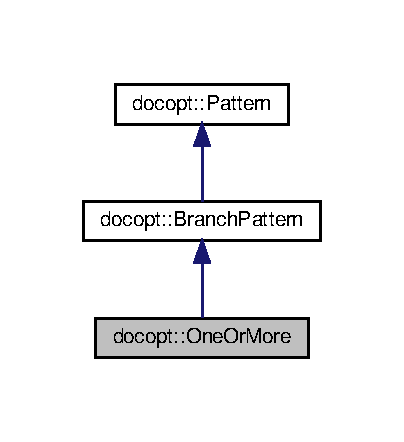
\includegraphics[width=194pt]{classdocopt_1_1OneOrMore__inherit__graph}
\end{center}
\end{figure}


Collaboration diagram for docopt\+:\+:One\+Or\+More\+:
\nopagebreak
\begin{figure}[H]
\begin{center}
\leavevmode
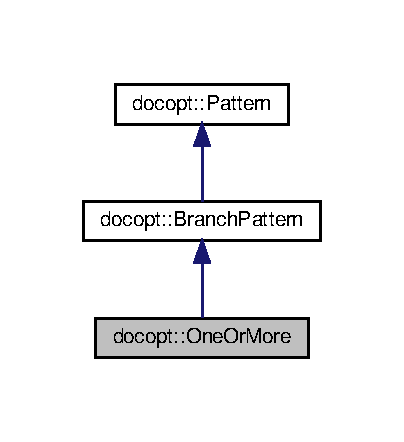
\includegraphics[width=194pt]{classdocopt_1_1OneOrMore__coll__graph}
\end{center}
\end{figure}
\subsection*{Public Member Functions}
\begin{DoxyCompactItemize}
\item 
\mbox{\Hypertarget{classdocopt_1_1OneOrMore_a9a381cacffb24af701a9e9283464fc23}\label{classdocopt_1_1OneOrMore_a9a381cacffb24af701a9e9283464fc23}} 
bool {\bfseries match} (Pattern\+List \&left, std\+::vector$<$ std\+::shared\+\_\+ptr$<$ \hyperlink{classdocopt_1_1LeafPattern}{Leaf\+Pattern} $>$$>$ \&collected) const override
\end{DoxyCompactItemize}
\subsection*{Additional Inherited Members}


The documentation for this class was generated from the following file\+:\begin{DoxyCompactItemize}
\item 
src/docopt\+\_\+cpp/docopt\+\_\+private.\+h\end{DoxyCompactItemize}

\hypertarget{classdocopt_1_1Option}{}\section{docopt\+:\+:Option Class Reference}
\label{classdocopt_1_1Option}\index{docopt\+::\+Option@{docopt\+::\+Option}}


Inheritance diagram for docopt\+:\+:Option\+:
% FIG 0


Collaboration diagram for docopt\+:\+:Option\+:
% FIG 1
\subsection*{Public Member Functions}
\begin{DoxyCompactItemize}
\item 
\mbox{\Hypertarget{classdocopt_1_1Option_a1da09cf8c24b9e40450f5d22ec26502d}\label{classdocopt_1_1Option_a1da09cf8c24b9e40450f5d22ec26502d}} 
{\bfseries Option} (std\+::string short\+Option, std\+::string long\+Option, int argcount=0, \hyperlink{structdocopt_1_1value}{value} v=\hyperlink{structdocopt_1_1value}{value}\{false\})
\item 
\mbox{\Hypertarget{classdocopt_1_1Option_af3996b856bd191cf0712ed34fa916f07}\label{classdocopt_1_1Option_af3996b856bd191cf0712ed34fa916f07}} 
{\bfseries Option} (\hyperlink{classdocopt_1_1Option}{Option} const \&)=default
\item 
\mbox{\Hypertarget{classdocopt_1_1Option_ac3860cc101da72b4309d6e58646c1441}\label{classdocopt_1_1Option_ac3860cc101da72b4309d6e58646c1441}} 
{\bfseries Option} (\hyperlink{classdocopt_1_1Option}{Option} \&\&)=default
\item 
\mbox{\Hypertarget{classdocopt_1_1Option_a48eaf5c2cf58bcdca3246692ec50248f}\label{classdocopt_1_1Option_a48eaf5c2cf58bcdca3246692ec50248f}} 
\hyperlink{classdocopt_1_1Option}{Option} \& {\bfseries operator=} (\hyperlink{classdocopt_1_1Option}{Option} const \&)=default
\item 
\mbox{\Hypertarget{classdocopt_1_1Option_acdfcb2a8b52d42ad94d756208141beb7}\label{classdocopt_1_1Option_acdfcb2a8b52d42ad94d756208141beb7}} 
\hyperlink{classdocopt_1_1Option}{Option} \& {\bfseries operator=} (\hyperlink{classdocopt_1_1Option}{Option} \&\&)=default
\item 
\mbox{\Hypertarget{classdocopt_1_1Option_ab7d5c918813d3c5414ff418bab3ed6e9}\label{classdocopt_1_1Option_ab7d5c918813d3c5414ff418bab3ed6e9}} 
std\+::string const  \& {\bfseries long\+Option} () const
\item 
\mbox{\Hypertarget{classdocopt_1_1Option_a7c1a506e66873d965dbb97dfd165b295}\label{classdocopt_1_1Option_a7c1a506e66873d965dbb97dfd165b295}} 
std\+::string const  \& {\bfseries short\+Option} () const
\item 
\mbox{\Hypertarget{classdocopt_1_1Option_a76ef24dea8376a828eeb53daadc3c1dd}\label{classdocopt_1_1Option_a76ef24dea8376a828eeb53daadc3c1dd}} 
int {\bfseries arg\+Count} () const
\item 
\mbox{\Hypertarget{classdocopt_1_1Option_a98ea6657e77e1f78baaace69486bef6a}\label{classdocopt_1_1Option_a98ea6657e77e1f78baaace69486bef6a}} 
virtual size\+\_\+t {\bfseries hash} () const override
\end{DoxyCompactItemize}
\subsection*{Static Public Member Functions}
\begin{DoxyCompactItemize}
\item 
\mbox{\Hypertarget{classdocopt_1_1Option_a49f14de794c19528b07cd6f39604a1a5}\label{classdocopt_1_1Option_a49f14de794c19528b07cd6f39604a1a5}} 
static \hyperlink{classdocopt_1_1Option}{Option} {\bfseries parse} (std\+::string const \&option\+\_\+description)
\end{DoxyCompactItemize}
\subsection*{Protected Member Functions}
\begin{DoxyCompactItemize}
\item 
\mbox{\Hypertarget{classdocopt_1_1Option_a8b395e69aa9718c6373330c8e29d3743}\label{classdocopt_1_1Option_a8b395e69aa9718c6373330c8e29d3743}} 
virtual std\+::pair$<$ size\+\_\+t, std\+::shared\+\_\+ptr$<$ \hyperlink{classdocopt_1_1LeafPattern}{Leaf\+Pattern} $>$ $>$ {\bfseries single\+\_\+match} (Pattern\+List const \&left) const override
\end{DoxyCompactItemize}


The documentation for this class was generated from the following file\+:\begin{DoxyCompactItemize}
\item 
src/docopt\+\_\+cpp/docopt\+\_\+private.\+h\end{DoxyCompactItemize}

\hypertarget{classdocopt_1_1Optional}{}\section{docopt\+:\+:Optional Class Reference}
\label{classdocopt_1_1Optional}\index{docopt\+::\+Optional@{docopt\+::\+Optional}}


Inheritance diagram for docopt\+:\+:Optional\+:
\nopagebreak
\begin{figure}[H]
\begin{center}
\leavevmode
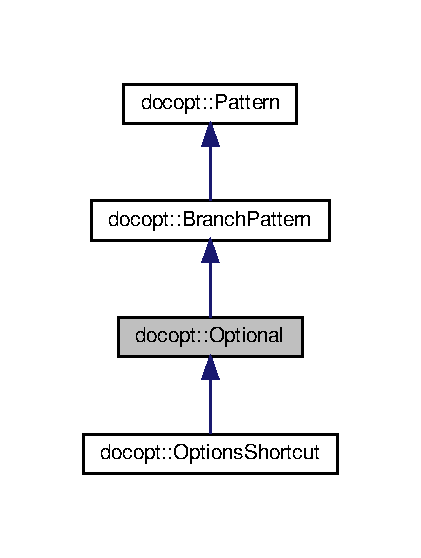
\includegraphics[width=202pt]{classdocopt_1_1Optional__inherit__graph}
\end{center}
\end{figure}


Collaboration diagram for docopt\+:\+:Optional\+:
\nopagebreak
\begin{figure}[H]
\begin{center}
\leavevmode
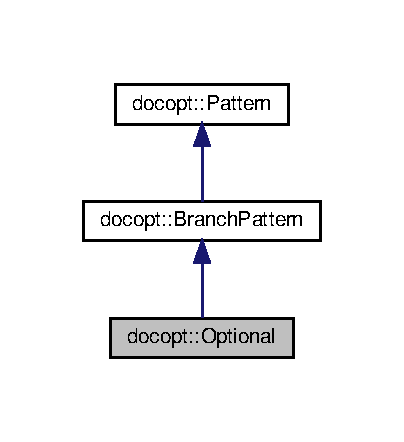
\includegraphics[width=194pt]{classdocopt_1_1Optional__coll__graph}
\end{center}
\end{figure}
\subsection*{Public Member Functions}
\begin{DoxyCompactItemize}
\item 
\mbox{\Hypertarget{classdocopt_1_1Optional_a64812d6b139119fb065b740099d7448d}\label{classdocopt_1_1Optional_a64812d6b139119fb065b740099d7448d}} 
bool {\bfseries match} (Pattern\+List \&left, std\+::vector$<$ std\+::shared\+\_\+ptr$<$ \hyperlink{classdocopt_1_1LeafPattern}{Leaf\+Pattern} $>$$>$ \&collected) const override
\end{DoxyCompactItemize}
\subsection*{Additional Inherited Members}


The documentation for this class was generated from the following file\+:\begin{DoxyCompactItemize}
\item 
src/docopt\+\_\+cpp/docopt\+\_\+private.\+h\end{DoxyCompactItemize}

\hypertarget{structTokens_1_1OptionError}{}\section{Tokens\+:\+:Option\+Error Struct Reference}
\label{structTokens_1_1OptionError}\index{Tokens\+::\+Option\+Error@{Tokens\+::\+Option\+Error}}


Inheritance diagram for Tokens\+:\+:Option\+Error\+:
\nopagebreak
\begin{figure}[H]
\begin{center}
\leavevmode
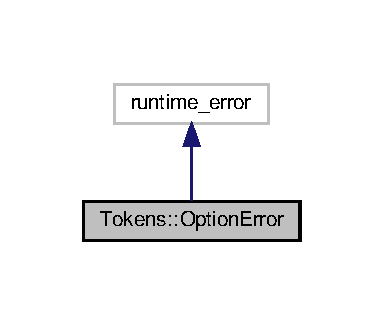
\includegraphics[width=184pt]{structTokens_1_1OptionError__inherit__graph}
\end{center}
\end{figure}


Collaboration diagram for Tokens\+:\+:Option\+Error\+:
\nopagebreak
\begin{figure}[H]
\begin{center}
\leavevmode
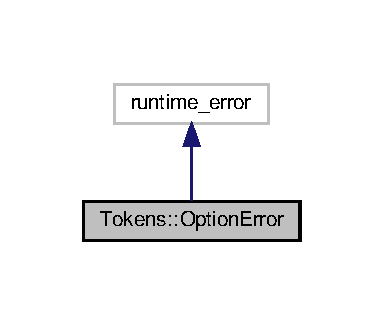
\includegraphics[width=184pt]{structTokens_1_1OptionError__coll__graph}
\end{center}
\end{figure}


The documentation for this struct was generated from the following file\+:\begin{DoxyCompactItemize}
\item 
src/docopt\+\_\+cpp/docopt.\+cpp\end{DoxyCompactItemize}

\hypertarget{classdocopt_1_1OptionsShortcut}{}\section{docopt\+:\+:Options\+Shortcut Class Reference}
\label{classdocopt_1_1OptionsShortcut}\index{docopt\+::\+Options\+Shortcut@{docopt\+::\+Options\+Shortcut}}


Inheritance diagram for docopt\+:\+:Options\+Shortcut\+:
\nopagebreak
\begin{figure}[H]
\begin{center}
\leavevmode
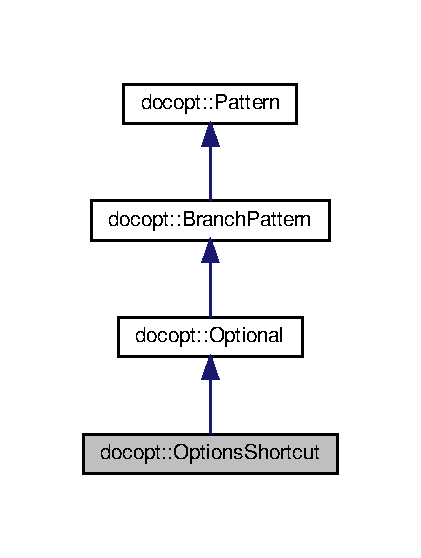
\includegraphics[width=202pt]{classdocopt_1_1OptionsShortcut__inherit__graph}
\end{center}
\end{figure}


Collaboration diagram for docopt\+:\+:Options\+Shortcut\+:
\nopagebreak
\begin{figure}[H]
\begin{center}
\leavevmode
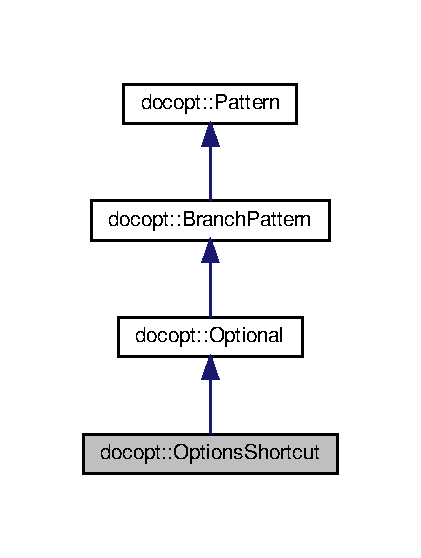
\includegraphics[width=202pt]{classdocopt_1_1OptionsShortcut__coll__graph}
\end{center}
\end{figure}
\subsection*{Additional Inherited Members}


The documentation for this class was generated from the following file\+:\begin{DoxyCompactItemize}
\item 
src/docopt\+\_\+cpp/docopt\+\_\+private.\+h\end{DoxyCompactItemize}

\hypertarget{classffft_1_1OscSinCos}{}\section{ffft\+:\+:Osc\+Sin\+Cos$<$ T $>$ Class Template Reference}
\label{classffft_1_1OscSinCos}\index{ffft\+::\+Osc\+Sin\+Cos$<$ T $>$@{ffft\+::\+Osc\+Sin\+Cos$<$ T $>$}}
\subsection*{Public Types}
\begin{DoxyCompactItemize}
\item 
\mbox{\Hypertarget{classffft_1_1OscSinCos_af91237051e92ce0af7aaf38b1826244d}\label{classffft_1_1OscSinCos_af91237051e92ce0af7aaf38b1826244d}} 
typedef T {\bfseries Data\+Type}
\end{DoxyCompactItemize}
\subsection*{Public Member Functions}
\begin{DoxyCompactItemize}
\item 
\mbox{\Hypertarget{classffft_1_1OscSinCos_ad41139a76b16a5af136d1e730a9143dc}\label{classffft_1_1OscSinCos_ad41139a76b16a5af136d1e730a9143dc}} 
ffft\+\_\+\+F\+O\+R\+C\+E\+I\+N\+L\+I\+NE void {\bfseries set\+\_\+step} (double angle\+\_\+rad)
\item 
\mbox{\Hypertarget{classffft_1_1OscSinCos_a88766d022a8e0067f987c170b9afd68a}\label{classffft_1_1OscSinCos_a88766d022a8e0067f987c170b9afd68a}} 
ffft\+\_\+\+F\+O\+R\+C\+E\+I\+N\+L\+I\+NE Data\+Type {\bfseries get\+\_\+cos} () const
\item 
\mbox{\Hypertarget{classffft_1_1OscSinCos_a842c33c2ed314cf62be6d273af00c416}\label{classffft_1_1OscSinCos_a842c33c2ed314cf62be6d273af00c416}} 
ffft\+\_\+\+F\+O\+R\+C\+E\+I\+N\+L\+I\+NE Data\+Type {\bfseries get\+\_\+sin} () const
\item 
\mbox{\Hypertarget{classffft_1_1OscSinCos_a442975ce6388271ea78998c080364e08}\label{classffft_1_1OscSinCos_a442975ce6388271ea78998c080364e08}} 
ffft\+\_\+\+F\+O\+R\+C\+E\+I\+N\+L\+I\+NE void {\bfseries step} ()
\item 
\mbox{\Hypertarget{classffft_1_1OscSinCos_a1be4a9ec10517ae2615d2925c05d7d29}\label{classffft_1_1OscSinCos_a1be4a9ec10517ae2615d2925c05d7d29}} 
ffft\+\_\+\+F\+O\+R\+C\+E\+I\+N\+L\+I\+NE void {\bfseries clear\+\_\+buffers} ()
\end{DoxyCompactItemize}


The documentation for this class was generated from the following files\+:\begin{DoxyCompactItemize}
\item 
src/include/ffft/Osc\+Sin\+Cos.\+h\item 
src/include/ffft/Osc\+Sin\+Cos.\+hpp\end{DoxyCompactItemize}

\hypertarget{classupc_1_1Path}{}\section{upc\+:\+:Path Class Reference}
\label{classupc_1_1Path}\index{upc\+::\+Path@{upc\+::\+Path}}


Inheritance diagram for upc\+:\+:Path\+:
\nopagebreak
\begin{figure}[H]
\begin{center}
\leavevmode
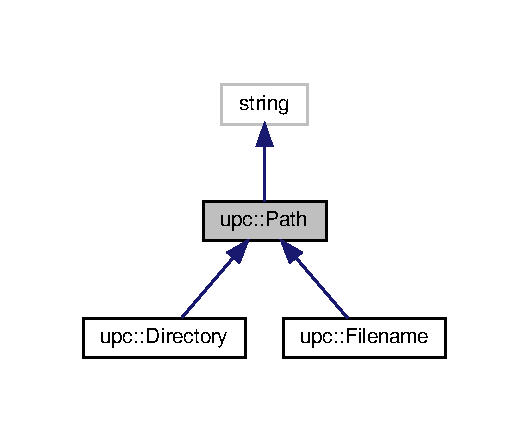
\includegraphics[width=254pt]{classupc_1_1Path__inherit__graph}
\end{center}
\end{figure}


Collaboration diagram for upc\+:\+:Path\+:
\nopagebreak
\begin{figure}[H]
\begin{center}
\leavevmode
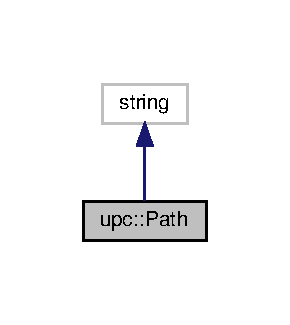
\includegraphics[width=139pt]{classupc_1_1Path__coll__graph}
\end{center}
\end{figure}
\subsection*{Public Member Functions}
\begin{DoxyCompactItemize}
\item 
\mbox{\Hypertarget{classupc_1_1Path_a364200f9a453fedd5ba68f79f8b93154}\label{classupc_1_1Path_a364200f9a453fedd5ba68f79f8b93154}} 
{\bfseries Path} (const string \&str)
\item 
\mbox{\Hypertarget{classupc_1_1Path_a082270e960275af46d65c3ce252ef581}\label{classupc_1_1Path_a082270e960275af46d65c3ce252ef581}} 
{\bfseries Path} (const char $\ast$str)
\end{DoxyCompactItemize}


The documentation for this class was generated from the following file\+:\begin{DoxyCompactItemize}
\item 
src/include/filename.\+h\end{DoxyCompactItemize}

\hypertarget{classdocopt_1_1Pattern}{}\section{docopt\+:\+:Pattern Class Reference}
\label{classdocopt_1_1Pattern}\index{docopt\+::\+Pattern@{docopt\+::\+Pattern}}


Inheritance diagram for docopt\+:\+:Pattern\+:
\nopagebreak
\begin{figure}[H]
\begin{center}
\leavevmode
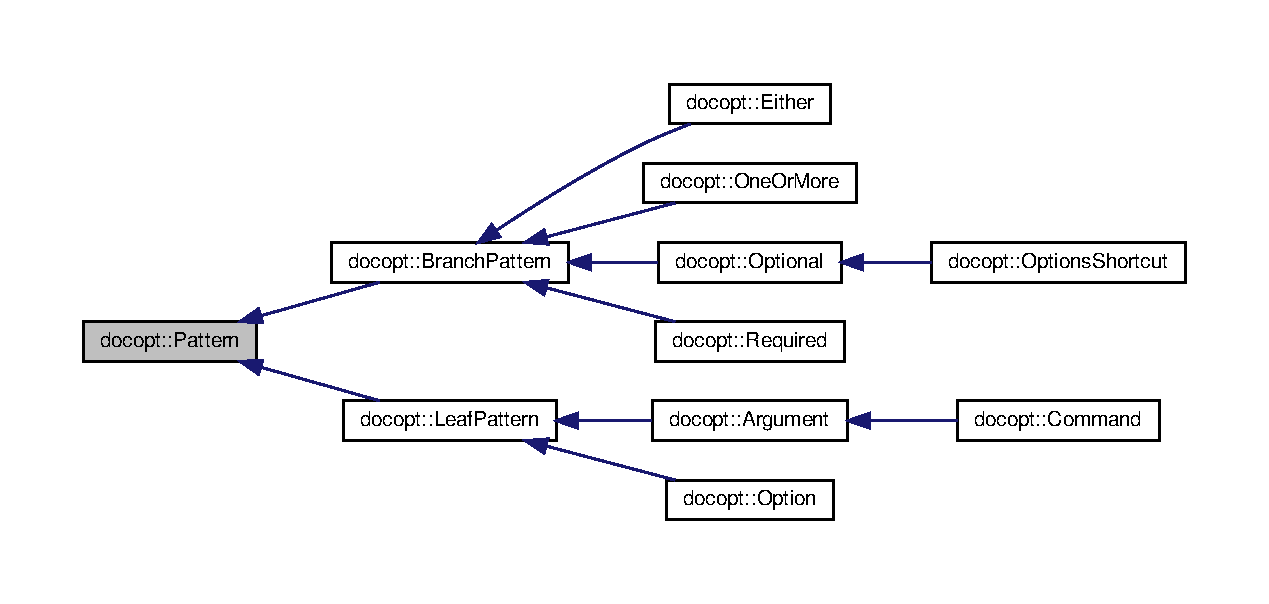
\includegraphics[width=350pt]{classdocopt_1_1Pattern__inherit__graph}
\end{center}
\end{figure}
\subsection*{Public Member Functions}
\begin{DoxyCompactItemize}
\item 
\mbox{\Hypertarget{classdocopt_1_1Pattern_a0a235229a02694f2127df05a890dec94}\label{classdocopt_1_1Pattern_a0a235229a02694f2127df05a890dec94}} 
virtual std\+::vector$<$ \hyperlink{classdocopt_1_1Pattern}{Pattern} $\ast$ $>$ {\bfseries flat} (bool($\ast$filter)(\hyperlink{classdocopt_1_1Pattern}{Pattern} const $\ast$))=0
\item 
\mbox{\Hypertarget{classdocopt_1_1Pattern_a6a16e61f7fc1634ff90b23aaf4336e2f}\label{classdocopt_1_1Pattern_a6a16e61f7fc1634ff90b23aaf4336e2f}} 
virtual void {\bfseries collect\+\_\+leaves} (std\+::vector$<$ \hyperlink{classdocopt_1_1LeafPattern}{Leaf\+Pattern} $\ast$$>$ \&)=0
\item 
\mbox{\Hypertarget{classdocopt_1_1Pattern_ae85dc8111e7786da5f19077d803683cb}\label{classdocopt_1_1Pattern_ae85dc8111e7786da5f19077d803683cb}} 
std\+::vector$<$ \hyperlink{classdocopt_1_1LeafPattern}{Leaf\+Pattern} $\ast$ $>$ {\bfseries leaves} ()
\item 
\mbox{\Hypertarget{classdocopt_1_1Pattern_abc6c22c0858f5a02be93530dc5e5c340}\label{classdocopt_1_1Pattern_abc6c22c0858f5a02be93530dc5e5c340}} 
virtual bool {\bfseries match} (Pattern\+List \&left, std\+::vector$<$ std\+::shared\+\_\+ptr$<$ \hyperlink{classdocopt_1_1LeafPattern}{Leaf\+Pattern} $>$$>$ \&collected) const =0
\item 
\mbox{\Hypertarget{classdocopt_1_1Pattern_a2334b803066089f752f75dfb8b6e6791}\label{classdocopt_1_1Pattern_a2334b803066089f752f75dfb8b6e6791}} 
virtual std\+::string const  \& {\bfseries name} () const =0
\item 
\mbox{\Hypertarget{classdocopt_1_1Pattern_a952fcee01661ea94019fdcbe168005a7}\label{classdocopt_1_1Pattern_a952fcee01661ea94019fdcbe168005a7}} 
virtual bool {\bfseries has\+Value} () const
\item 
\mbox{\Hypertarget{classdocopt_1_1Pattern_a4fdb3144b57b5a9350529c42878f1578}\label{classdocopt_1_1Pattern_a4fdb3144b57b5a9350529c42878f1578}} 
virtual size\+\_\+t {\bfseries hash} () const =0
\end{DoxyCompactItemize}


The documentation for this class was generated from the following file\+:\begin{DoxyCompactItemize}
\item 
src/docopt\+\_\+cpp/docopt\+\_\+private.\+h\end{DoxyCompactItemize}

\hypertarget{structdocopt_1_1PatternHasher}{}\section{docopt\+:\+:Pattern\+Hasher Struct Reference}
\label{structdocopt_1_1PatternHasher}\index{docopt\+::\+Pattern\+Hasher@{docopt\+::\+Pattern\+Hasher}}
\subsection*{Public Member Functions}
\begin{DoxyCompactItemize}
\item 
\mbox{\Hypertarget{structdocopt_1_1PatternHasher_a1710a6bd411652415e3fb887f543a59e}\label{structdocopt_1_1PatternHasher_a1710a6bd411652415e3fb887f543a59e}} 
{\footnotesize template$<$typename P $>$ }\\size\+\_\+t {\bfseries operator()} (std\+::shared\+\_\+ptr$<$ P $>$ const \&pattern) const
\item 
\mbox{\Hypertarget{structdocopt_1_1PatternHasher_a4d2b0b65ac3f809a34557fc4dd35afc2}\label{structdocopt_1_1PatternHasher_a4d2b0b65ac3f809a34557fc4dd35afc2}} 
{\footnotesize template$<$typename P $>$ }\\size\+\_\+t {\bfseries operator()} (P const $\ast$pattern) const
\item 
\mbox{\Hypertarget{structdocopt_1_1PatternHasher_ab5f6cd063dd6a0c767e8d79e47af4450}\label{structdocopt_1_1PatternHasher_ab5f6cd063dd6a0c767e8d79e47af4450}} 
{\footnotesize template$<$typename P $>$ }\\size\+\_\+t {\bfseries operator()} (P const \&pattern) const
\end{DoxyCompactItemize}


The documentation for this struct was generated from the following file\+:\begin{DoxyCompactItemize}
\item 
src/docopt\+\_\+cpp/docopt\+\_\+private.\+h\end{DoxyCompactItemize}

\hypertarget{structdocopt_1_1PatternPointerEquality}{}\section{docopt\+:\+:Pattern\+Pointer\+Equality Struct Reference}
\label{structdocopt_1_1PatternPointerEquality}\index{docopt\+::\+Pattern\+Pointer\+Equality@{docopt\+::\+Pattern\+Pointer\+Equality}}
\subsection*{Public Member Functions}
\begin{DoxyCompactItemize}
\item 
\mbox{\Hypertarget{structdocopt_1_1PatternPointerEquality_a9e18a6a036f66503b9426f51210370d3}\label{structdocopt_1_1PatternPointerEquality_a9e18a6a036f66503b9426f51210370d3}} 
{\footnotesize template$<$typename P1 , typename P2 $>$ }\\bool {\bfseries operator()} (std\+::shared\+\_\+ptr$<$ P1 $>$ const \&p1, std\+::shared\+\_\+ptr$<$ P2 $>$ const \&p2) const
\item 
\mbox{\Hypertarget{structdocopt_1_1PatternPointerEquality_a7253b1900c027275af33d0905a8adfcf}\label{structdocopt_1_1PatternPointerEquality_a7253b1900c027275af33d0905a8adfcf}} 
{\footnotesize template$<$typename P1 , typename P2 $>$ }\\bool {\bfseries operator()} (P1 const $\ast$p1, P2 const $\ast$p2) const
\end{DoxyCompactItemize}


The documentation for this struct was generated from the following file\+:\begin{DoxyCompactItemize}
\item 
src/docopt\+\_\+cpp/docopt\+\_\+private.\+h\end{DoxyCompactItemize}

\hypertarget{classupc_1_1PitchAnalyzer}{}\section{upc\+:\+:Pitch\+Analyzer Class Reference}
\label{classupc_1_1PitchAnalyzer}\index{upc\+::\+Pitch\+Analyzer@{upc\+::\+Pitch\+Analyzer}}


{\ttfamily \#include $<$pitch\+\_\+analyzer.\+h$>$}

\subsection*{Public Types}
\begin{DoxyCompactItemize}
\item 
enum \hyperlink{classupc_1_1PitchAnalyzer_ab82b7694d6bc72839e5be6e526be81b6}{Window} \{ \hyperlink{classupc_1_1PitchAnalyzer_ab82b7694d6bc72839e5be6e526be81b6ae89513dddf240af8bbef3358597f244c}{R\+E\+CT}, 
\hyperlink{classupc_1_1PitchAnalyzer_ab82b7694d6bc72839e5be6e526be81b6a20e793e736a503aacbed0294970a9b33}{H\+A\+M\+M\+I\+NG}
 \}\begin{DoxyCompactList}\small\item\em Wndow type. \end{DoxyCompactList}
\end{DoxyCompactItemize}
\subsection*{Public Member Functions}
\begin{DoxyCompactItemize}
\item 
void \hyperlink{classupc_1_1PitchAnalyzer_a96cc042a650825b25ca39c41beebd0db}{set\+\_\+window} (\hyperlink{classupc_1_1PitchAnalyzer_ab82b7694d6bc72839e5be6e526be81b6}{Window} type)
\begin{DoxyCompactList}\small\item\em pre-\/compute window \end{DoxyCompactList}\item 
\hyperlink{classupc_1_1PitchAnalyzer_ae7cfb918feadd7d56f5736e4ef600c06}{Pitch\+Analyzer} (unsigned int f\+Len, unsigned int s\+Freq, \hyperlink{classupc_1_1PitchAnalyzer_ab82b7694d6bc72839e5be6e526be81b6}{Window} w=\hyperlink{classupc_1_1PitchAnalyzer_ab82b7694d6bc72839e5be6e526be81b6a20e793e736a503aacbed0294970a9b33}{Pitch\+Analyzer\+::\+H\+A\+M\+M\+I\+NG}, float min\+\_\+\+F0=\hyperlink{namespaceupc_ae8ed4ce6dc2c05dfc1aa6432db41e1ae}{M\+I\+N\+\_\+\+F0}, float max\+\_\+\+F0=\hyperlink{namespaceupc_ab69be42753266b6e1a0deaa8eba56a19}{M\+A\+X\+\_\+\+F0})
\item 
float \hyperlink{classupc_1_1PitchAnalyzer_a96e4ab38ac616924ac464d77481dfc84}{operator()} (const std\+::vector$<$ float $>$ \&\+\_\+x) const
\item 
float \hyperlink{classupc_1_1PitchAnalyzer_ac4fe50035ebbb1602ab9f4c90755ba0a}{operator()} (const float $\ast$pt, unsigned int N) const
\item 
float \hyperlink{classupc_1_1PitchAnalyzer_a6ae2aaad64d2768c7869f01d25e9d5e6}{operator()} (std\+::vector$<$ float $>$\+::const\+\_\+iterator begin, std\+::vector$<$ float $>$\+::const\+\_\+iterator end) const
\item 
void \hyperlink{classupc_1_1PitchAnalyzer_ac33887654b62b3f90c3de231ec187d94}{set\+\_\+f0\+\_\+range} (float min\+\_\+\+F0, float max\+\_\+\+F0)
\end{DoxyCompactItemize}


\subsection{Detailed Description}
\hyperlink{classupc_1_1PitchAnalyzer}{Pitch\+Analyzer}\+: class that computes the pitch (in Hz) from a signal frame. No pre-\/processing or post-\/processing has been included 

\subsection{Member Enumeration Documentation}
\mbox{\Hypertarget{classupc_1_1PitchAnalyzer_ab82b7694d6bc72839e5be6e526be81b6}\label{classupc_1_1PitchAnalyzer_ab82b7694d6bc72839e5be6e526be81b6}} 
\index{upc\+::\+Pitch\+Analyzer@{upc\+::\+Pitch\+Analyzer}!Window@{Window}}
\index{Window@{Window}!upc\+::\+Pitch\+Analyzer@{upc\+::\+Pitch\+Analyzer}}
\subsubsection{\texorpdfstring{Window}{Window}}
{\footnotesize\ttfamily enum \hyperlink{classupc_1_1PitchAnalyzer_ab82b7694d6bc72839e5be6e526be81b6}{upc\+::\+Pitch\+Analyzer\+::\+Window}}



Wndow type. 

\begin{DoxyEnumFields}{Enumerator}
\raisebox{\heightof{T}}[0pt][0pt]{\index{R\+E\+CT@{R\+E\+CT}!upc\+::\+Pitch\+Analyzer@{upc\+::\+Pitch\+Analyzer}}\index{upc\+::\+Pitch\+Analyzer@{upc\+::\+Pitch\+Analyzer}!R\+E\+CT@{R\+E\+CT}}}\mbox{\Hypertarget{classupc_1_1PitchAnalyzer_ab82b7694d6bc72839e5be6e526be81b6ae89513dddf240af8bbef3358597f244c}\label{classupc_1_1PitchAnalyzer_ab82b7694d6bc72839e5be6e526be81b6ae89513dddf240af8bbef3358597f244c}} 
R\+E\+CT&Rectangular window. \\
\hline

\raisebox{\heightof{T}}[0pt][0pt]{\index{H\+A\+M\+M\+I\+NG@{H\+A\+M\+M\+I\+NG}!upc\+::\+Pitch\+Analyzer@{upc\+::\+Pitch\+Analyzer}}\index{upc\+::\+Pitch\+Analyzer@{upc\+::\+Pitch\+Analyzer}!H\+A\+M\+M\+I\+NG@{H\+A\+M\+M\+I\+NG}}}\mbox{\Hypertarget{classupc_1_1PitchAnalyzer_ab82b7694d6bc72839e5be6e526be81b6a20e793e736a503aacbed0294970a9b33}\label{classupc_1_1PitchAnalyzer_ab82b7694d6bc72839e5be6e526be81b6a20e793e736a503aacbed0294970a9b33}} 
H\+A\+M\+M\+I\+NG&Hamming window. \\
\hline

\end{DoxyEnumFields}


\subsection{Constructor \& Destructor Documentation}
\mbox{\Hypertarget{classupc_1_1PitchAnalyzer_ae7cfb918feadd7d56f5736e4ef600c06}\label{classupc_1_1PitchAnalyzer_ae7cfb918feadd7d56f5736e4ef600c06}} 
\index{upc\+::\+Pitch\+Analyzer@{upc\+::\+Pitch\+Analyzer}!Pitch\+Analyzer@{Pitch\+Analyzer}}
\index{Pitch\+Analyzer@{Pitch\+Analyzer}!upc\+::\+Pitch\+Analyzer@{upc\+::\+Pitch\+Analyzer}}
\subsubsection{\texorpdfstring{Pitch\+Analyzer()}{PitchAnalyzer()}}
{\footnotesize\ttfamily upc\+::\+Pitch\+Analyzer\+::\+Pitch\+Analyzer (\begin{DoxyParamCaption}\item[{unsigned int}]{f\+Len,  }\item[{unsigned int}]{s\+Freq,  }\item[{\hyperlink{classupc_1_1PitchAnalyzer_ab82b7694d6bc72839e5be6e526be81b6}{Window}}]{w = {\ttfamily \hyperlink{classupc_1_1PitchAnalyzer_ab82b7694d6bc72839e5be6e526be81b6a20e793e736a503aacbed0294970a9b33}{Pitch\+Analyzer\+::\+H\+A\+M\+M\+I\+NG}},  }\item[{float}]{min\+\_\+\+F0 = {\ttfamily \hyperlink{namespaceupc_ae8ed4ce6dc2c05dfc1aa6432db41e1ae}{M\+I\+N\+\_\+\+F0}},  }\item[{float}]{max\+\_\+\+F0 = {\ttfamily \hyperlink{namespaceupc_ab69be42753266b6e1a0deaa8eba56a19}{M\+A\+X\+\_\+\+F0}} }\end{DoxyParamCaption})\hspace{0.3cm}{\ttfamily [inline]}}


\begin{DoxyParams}{Parameters}
{\em f\+Len} & Frame length in samples \\
\hline
{\em s\+Freq} & Sampling rate in Hertzs \\
\hline
{\em w} & Window type \\
\hline
{\em min\+\_\+\+F0} & Pitch range should be restricted to be above this value \\
\hline
{\em max\+\_\+\+F0} & Pitch range should be restricted to be below this value \\
\hline
\end{DoxyParams}


\subsection{Member Function Documentation}
\mbox{\Hypertarget{classupc_1_1PitchAnalyzer_a96e4ab38ac616924ac464d77481dfc84}\label{classupc_1_1PitchAnalyzer_a96e4ab38ac616924ac464d77481dfc84}} 
\index{upc\+::\+Pitch\+Analyzer@{upc\+::\+Pitch\+Analyzer}!operator()@{operator()}}
\index{operator()@{operator()}!upc\+::\+Pitch\+Analyzer@{upc\+::\+Pitch\+Analyzer}}
\subsubsection{\texorpdfstring{operator()()}{operator()()}\hspace{0.1cm}{\footnotesize\ttfamily [1/3]}}
{\footnotesize\ttfamily float upc\+::\+Pitch\+Analyzer\+::operator() (\begin{DoxyParamCaption}\item[{const std\+::vector$<$ float $>$ \&}]{\+\_\+x }\end{DoxyParamCaption}) const\hspace{0.3cm}{\ttfamily [inline]}}

Operator ()\+: computes the pitch for the given vector x \mbox{\Hypertarget{classupc_1_1PitchAnalyzer_ac4fe50035ebbb1602ab9f4c90755ba0a}\label{classupc_1_1PitchAnalyzer_ac4fe50035ebbb1602ab9f4c90755ba0a}} 
\index{upc\+::\+Pitch\+Analyzer@{upc\+::\+Pitch\+Analyzer}!operator()@{operator()}}
\index{operator()@{operator()}!upc\+::\+Pitch\+Analyzer@{upc\+::\+Pitch\+Analyzer}}
\subsubsection{\texorpdfstring{operator()()}{operator()()}\hspace{0.1cm}{\footnotesize\ttfamily [2/3]}}
{\footnotesize\ttfamily float upc\+::\+Pitch\+Analyzer\+::operator() (\begin{DoxyParamCaption}\item[{const float $\ast$}]{pt,  }\item[{unsigned int}]{N }\end{DoxyParamCaption}) const\hspace{0.3cm}{\ttfamily [inline]}}

Operator ()\+: computes the pitch for the given \char`\"{}\+C\char`\"{} vector (float $\ast$). N is the size of the vector pointer by pt. copy input values into local vector x \mbox{\Hypertarget{classupc_1_1PitchAnalyzer_a6ae2aaad64d2768c7869f01d25e9d5e6}\label{classupc_1_1PitchAnalyzer_a6ae2aaad64d2768c7869f01d25e9d5e6}} 
\index{upc\+::\+Pitch\+Analyzer@{upc\+::\+Pitch\+Analyzer}!operator()@{operator()}}
\index{operator()@{operator()}!upc\+::\+Pitch\+Analyzer@{upc\+::\+Pitch\+Analyzer}}
\subsubsection{\texorpdfstring{operator()()}{operator()()}\hspace{0.1cm}{\footnotesize\ttfamily [3/3]}}
{\footnotesize\ttfamily float upc\+::\+Pitch\+Analyzer\+::operator() (\begin{DoxyParamCaption}\item[{std\+::vector$<$ float $>$\+::const\+\_\+iterator}]{begin,  }\item[{std\+::vector$<$ float $>$\+::const\+\_\+iterator}]{end }\end{DoxyParamCaption}) const\hspace{0.3cm}{\ttfamily [inline]}}

Operator ()\+: computes the pitch for the given vector, expressed by the begin and end iterators \mbox{\Hypertarget{classupc_1_1PitchAnalyzer_ac33887654b62b3f90c3de231ec187d94}\label{classupc_1_1PitchAnalyzer_ac33887654b62b3f90c3de231ec187d94}} 
\index{upc\+::\+Pitch\+Analyzer@{upc\+::\+Pitch\+Analyzer}!set\+\_\+f0\+\_\+range@{set\+\_\+f0\+\_\+range}}
\index{set\+\_\+f0\+\_\+range@{set\+\_\+f0\+\_\+range}!upc\+::\+Pitch\+Analyzer@{upc\+::\+Pitch\+Analyzer}}
\subsubsection{\texorpdfstring{set\+\_\+f0\+\_\+range()}{set\_f0\_range()}}
{\footnotesize\ttfamily void upc\+::\+Pitch\+Analyzer\+::set\+\_\+f0\+\_\+range (\begin{DoxyParamCaption}\item[{float}]{min\+\_\+\+F0,  }\item[{float}]{max\+\_\+\+F0 }\end{DoxyParamCaption})}

Sets pitch range\+: takes min\+\_\+\+F0 and max\+\_\+\+F0 in Hz, sets npitch\+\_\+min and npitch\+\_\+max in samples \mbox{\Hypertarget{classupc_1_1PitchAnalyzer_a96cc042a650825b25ca39c41beebd0db}\label{classupc_1_1PitchAnalyzer_a96cc042a650825b25ca39c41beebd0db}} 
\index{upc\+::\+Pitch\+Analyzer@{upc\+::\+Pitch\+Analyzer}!set\+\_\+window@{set\+\_\+window}}
\index{set\+\_\+window@{set\+\_\+window}!upc\+::\+Pitch\+Analyzer@{upc\+::\+Pitch\+Analyzer}}
\subsubsection{\texorpdfstring{set\+\_\+window()}{set\_window()}}
{\footnotesize\ttfamily void upc\+::\+Pitch\+Analyzer\+::set\+\_\+window (\begin{DoxyParamCaption}\item[{\hyperlink{classupc_1_1PitchAnalyzer_ab82b7694d6bc72839e5be6e526be81b6}{Window}}]{type }\end{DoxyParamCaption})}



pre-\/compute window 

Implement the Hamming window 

The documentation for this class was generated from the following files\+:\begin{DoxyCompactItemize}
\item 
src/get\+\_\+pitch/\hyperlink{pitch__analyzer_8h}{pitch\+\_\+analyzer.\+h}\item 
src/get\+\_\+pitch/\hyperlink{pitch__analyzer_8cpp}{pitch\+\_\+analyzer.\+cpp}\end{DoxyCompactItemize}

\hypertarget{classdocopt_1_1Required}{}\section{docopt\+:\+:Required Class Reference}
\label{classdocopt_1_1Required}\index{docopt\+::\+Required@{docopt\+::\+Required}}


Inheritance diagram for docopt\+:\+:Required\+:
% FIG 0


Collaboration diagram for docopt\+:\+:Required\+:
% FIG 1
\subsection*{Public Member Functions}
\begin{DoxyCompactItemize}
\item 
\mbox{\Hypertarget{classdocopt_1_1Required_a83b4fcb821eebe551d5fdf3ff9703c97}\label{classdocopt_1_1Required_a83b4fcb821eebe551d5fdf3ff9703c97}} 
bool {\bfseries match} (Pattern\+List \&left, std\+::vector$<$ std\+::shared\+\_\+ptr$<$ \hyperlink{classdocopt_1_1LeafPattern}{Leaf\+Pattern} $>$$>$ \&collected) const override
\end{DoxyCompactItemize}
\subsection*{Additional Inherited Members}


The documentation for this class was generated from the following file\+:\begin{DoxyCompactItemize}
\item 
src/docopt\+\_\+cpp/docopt\+\_\+private.\+h\end{DoxyCompactItemize}

\hypertarget{classTokens}{}\section{Tokens Class Reference}
\label{classTokens}\index{Tokens@{Tokens}}
\subsection*{Classes}
\begin{DoxyCompactItemize}
\item 
struct \hyperlink{structTokens_1_1OptionError}{Option\+Error}
\end{DoxyCompactItemize}
\subsection*{Public Member Functions}
\begin{DoxyCompactItemize}
\item 
\mbox{\Hypertarget{classTokens_a6f319545790af24e81a9e811cbd01edb}\label{classTokens_a6f319545790af24e81a9e811cbd01edb}} 
{\bfseries Tokens} (std\+::vector$<$ std\+::string $>$ tokens, bool is\+Parsing\+Argv=true)
\item 
\mbox{\Hypertarget{classTokens_aedd895b4073f541ef319564c76b91c19}\label{classTokens_aedd895b4073f541ef319564c76b91c19}} 
{\bfseries operator bool} () const
\item 
\mbox{\Hypertarget{classTokens_acb0fda75975c72f45ca93b0236c3e65b}\label{classTokens_acb0fda75975c72f45ca93b0236c3e65b}} 
std\+::string const  \& {\bfseries current} () const
\item 
\mbox{\Hypertarget{classTokens_a642f50345bdc0cca8add2305dc44d0d7}\label{classTokens_a642f50345bdc0cca8add2305dc44d0d7}} 
std\+::string {\bfseries the\+\_\+rest} () const
\item 
\mbox{\Hypertarget{classTokens_ae07c89765c0406cdf25c638f5b98a070}\label{classTokens_ae07c89765c0406cdf25c638f5b98a070}} 
std\+::string {\bfseries pop} ()
\item 
\mbox{\Hypertarget{classTokens_a1efe979cd80d3af5559c9d7bf428e6e7}\label{classTokens_a1efe979cd80d3af5559c9d7bf428e6e7}} 
bool {\bfseries is\+Parsing\+Argv} () const
\end{DoxyCompactItemize}
\subsection*{Static Public Member Functions}
\begin{DoxyCompactItemize}
\item 
\mbox{\Hypertarget{classTokens_a16874c82bd94f507cd69bbf8ab342768}\label{classTokens_a16874c82bd94f507cd69bbf8ab342768}} 
static \hyperlink{classTokens}{Tokens} {\bfseries from\+\_\+pattern} (std\+::string const \&source)
\end{DoxyCompactItemize}


The documentation for this class was generated from the following file\+:\begin{DoxyCompactItemize}
\item 
src/docopt\+\_\+cpp/docopt.\+cpp\end{DoxyCompactItemize}

\hypertarget{structdocopt_1_1value}{}\section{docopt\+:\+:value Struct Reference}
\label{structdocopt_1_1value}\index{docopt\+::value@{docopt\+::value}}


{\ttfamily \#include $<$docopt\+\_\+value.\+h$>$}

\subsection*{Public Member Functions}
\begin{DoxyCompactItemize}
\item 
\mbox{\Hypertarget{structdocopt_1_1value_ab768a11740f6c251ed6207093f6dc066}\label{structdocopt_1_1value_ab768a11740f6c251ed6207093f6dc066}} 
\hyperlink{structdocopt_1_1value_ab768a11740f6c251ed6207093f6dc066}{value} ()
\begin{DoxyCompactList}\small\item\em An empty value. \end{DoxyCompactList}\item 
\mbox{\Hypertarget{structdocopt_1_1value_a35d519b82e27b7fe3aa008c046420204}\label{structdocopt_1_1value_a35d519b82e27b7fe3aa008c046420204}} 
{\bfseries value} (std\+::string)
\item 
\mbox{\Hypertarget{structdocopt_1_1value_a32dd6b7ac476b3a8b0a89bfb953f92dd}\label{structdocopt_1_1value_a32dd6b7ac476b3a8b0a89bfb953f92dd}} 
{\bfseries value} (std\+::vector$<$ std\+::string $>$)
\item 
\mbox{\Hypertarget{structdocopt_1_1value_ad86d6c1758e50c3d7717d182b14d87e4}\label{structdocopt_1_1value_ad86d6c1758e50c3d7717d182b14d87e4}} 
{\bfseries value} (bool)
\item 
\mbox{\Hypertarget{structdocopt_1_1value_a81883678cad49edea2992cea86397c02}\label{structdocopt_1_1value_a81883678cad49edea2992cea86397c02}} 
{\bfseries value} (long)
\item 
\mbox{\Hypertarget{structdocopt_1_1value_a39ece19eb013dfba4df75137a8c0781d}\label{structdocopt_1_1value_a39ece19eb013dfba4df75137a8c0781d}} 
{\bfseries value} (int v)
\item 
\mbox{\Hypertarget{structdocopt_1_1value_ad08e1a856e3e086edeaccc3dddb94fde}\label{structdocopt_1_1value_ad08e1a856e3e086edeaccc3dddb94fde}} 
{\bfseries value} (\hyperlink{structdocopt_1_1value}{value} const \&)
\item 
\mbox{\Hypertarget{structdocopt_1_1value_ac3710804ae623fa0e524c23524cc765c}\label{structdocopt_1_1value_ac3710804ae623fa0e524c23524cc765c}} 
{\bfseries value} (\hyperlink{structdocopt_1_1value}{value} \&\&) noexcept
\item 
\mbox{\Hypertarget{structdocopt_1_1value_a7d4caf9cee73181e601c552d91c67c83}\label{structdocopt_1_1value_a7d4caf9cee73181e601c552d91c67c83}} 
\hyperlink{structdocopt_1_1value}{value} \& {\bfseries operator=} (\hyperlink{structdocopt_1_1value}{value} const \&)
\item 
\mbox{\Hypertarget{structdocopt_1_1value_ad631e7d4d8abdf0263f03c5915a1e7f9}\label{structdocopt_1_1value_ad631e7d4d8abdf0263f03c5915a1e7f9}} 
\hyperlink{structdocopt_1_1value}{value} \& {\bfseries operator=} (\hyperlink{structdocopt_1_1value}{value} \&\&) noexcept
\item 
\mbox{\Hypertarget{structdocopt_1_1value_a781bbacfa45b53aa77159b00cbb344d8}\label{structdocopt_1_1value_a781bbacfa45b53aa77159b00cbb344d8}} 
{\bfseries operator bool} () const
\item 
\mbox{\Hypertarget{structdocopt_1_1value_ad426d707f8e8297151f01813827bc3ec}\label{structdocopt_1_1value_ad426d707f8e8297151f01813827bc3ec}} 
bool {\bfseries is\+Bool} () const
\item 
\mbox{\Hypertarget{structdocopt_1_1value_a18f3e2db1103c9a115e7c5155155b58c}\label{structdocopt_1_1value_a18f3e2db1103c9a115e7c5155155b58c}} 
bool {\bfseries is\+String} () const
\item 
\mbox{\Hypertarget{structdocopt_1_1value_af6b108aae989371310be8dcf1b84837a}\label{structdocopt_1_1value_af6b108aae989371310be8dcf1b84837a}} 
bool {\bfseries is\+Long} () const
\item 
\mbox{\Hypertarget{structdocopt_1_1value_af9eaafab4c25c572d14140e4fb0c38e2}\label{structdocopt_1_1value_af9eaafab4c25c572d14140e4fb0c38e2}} 
bool {\bfseries is\+String\+List} () const
\item 
\mbox{\Hypertarget{structdocopt_1_1value_a0f73668a1c8451d7e3471b1aebd4fa3d}\label{structdocopt_1_1value_a0f73668a1c8451d7e3471b1aebd4fa3d}} 
bool {\bfseries as\+Bool} () const
\item 
\mbox{\Hypertarget{structdocopt_1_1value_a4b3bf11b1f06c643f62a7ce842d49282}\label{structdocopt_1_1value_a4b3bf11b1f06c643f62a7ce842d49282}} 
long {\bfseries as\+Long} () const
\item 
\mbox{\Hypertarget{structdocopt_1_1value_a69aa7f940b1e8b3e5f8e283e80412475}\label{structdocopt_1_1value_a69aa7f940b1e8b3e5f8e283e80412475}} 
std\+::string const  \& {\bfseries as\+String} () const
\item 
\mbox{\Hypertarget{structdocopt_1_1value_af3f860f403f5c6d61eda6f7296a378c5}\label{structdocopt_1_1value_af3f860f403f5c6d61eda6f7296a378c5}} 
std\+::vector$<$ std\+::string $>$ const  \& {\bfseries as\+String\+List} () const
\item 
\mbox{\Hypertarget{structdocopt_1_1value_adf5870e74191ec2202bd26193147be79}\label{structdocopt_1_1value_adf5870e74191ec2202bd26193147be79}} 
size\+\_\+t {\bfseries hash} () const noexcept
\end{DoxyCompactItemize}
\subsection*{Friends}
\begin{DoxyCompactItemize}
\item 
\mbox{\Hypertarget{structdocopt_1_1value_a978098e745a3a42613ee4a31d6fc7a3d}\label{structdocopt_1_1value_a978098e745a3a42613ee4a31d6fc7a3d}} 
bool {\bfseries operator==} (\hyperlink{structdocopt_1_1value}{value} const \&, \hyperlink{structdocopt_1_1value}{value} const \&)
\item 
\mbox{\Hypertarget{structdocopt_1_1value_a12dc6286941afe66b4a5666ef515b194}\label{structdocopt_1_1value_a12dc6286941afe66b4a5666ef515b194}} 
bool {\bfseries operator!=} (\hyperlink{structdocopt_1_1value}{value} const \&, \hyperlink{structdocopt_1_1value}{value} const \&)
\end{DoxyCompactItemize}


\subsection{Detailed Description}
A generic type to hold the various types that can be produced by docopt.

This type can be one of\+: \{bool, long, string, vector$<$string$>$\}, or empty. 

The documentation for this struct was generated from the following file\+:\begin{DoxyCompactItemize}
\item 
src/docopt\+\_\+cpp/docopt\+\_\+value.\+h\end{DoxyCompactItemize}

\chapter{File Documentation}
\hypertarget{get__pitch_8cpp}{}\section{src/get\+\_\+pitch/get\+\_\+pitch.cpp File Reference}
\label{get__pitch_8cpp}\index{src/get\+\_\+pitch/get\+\_\+pitch.\+cpp@{src/get\+\_\+pitch/get\+\_\+pitch.\+cpp}}
{\ttfamily \#include $<$iostream$>$}\newline
{\ttfamily \#include $<$fstream$>$}\newline
{\ttfamily \#include $<$string.\+h$>$}\newline
{\ttfamily \#include $<$errno.\+h$>$}\newline
{\ttfamily \#include \char`\"{}wavfile\+\_\+mono.\+h\char`\"{}}\newline
{\ttfamily \#include \char`\"{}pitch\+\_\+analyzer.\+h\char`\"{}}\newline
{\ttfamily \#include \char`\"{}docopt.\+h\char`\"{}}\newline
Include dependency graph for get\+\_\+pitch.\+cpp\+:
\nopagebreak
\begin{figure}[H]
\begin{center}
\leavevmode
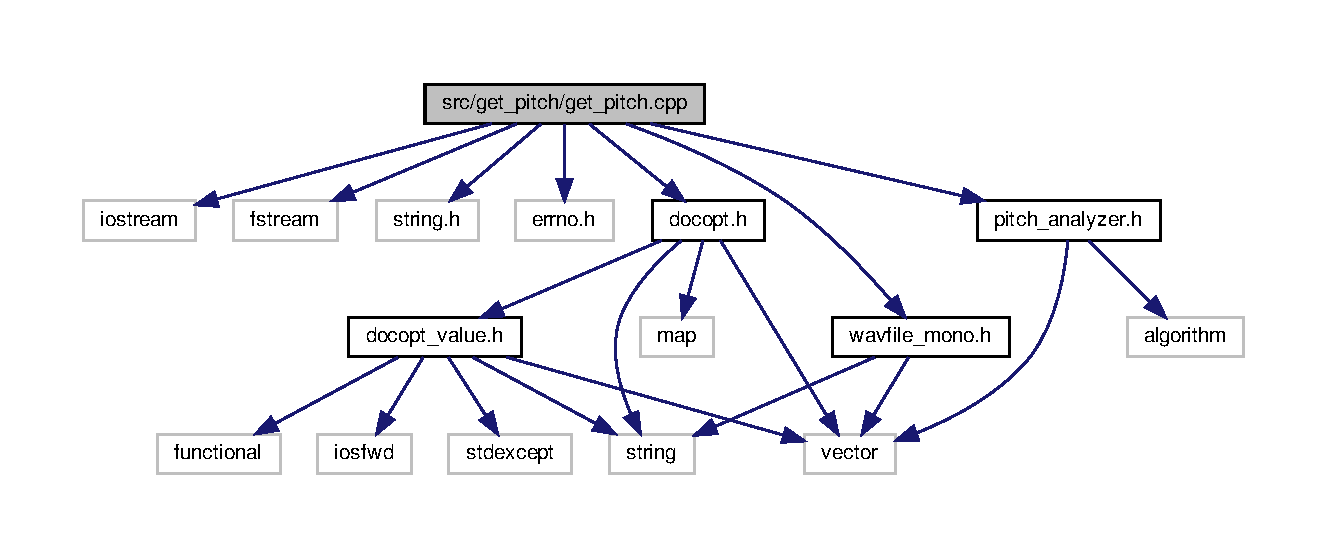
\includegraphics[width=350pt]{get__pitch_8cpp__incl}
\end{center}
\end{figure}
\subsection*{Macros}
\begin{DoxyCompactItemize}
\item 
\mbox{\Hypertarget{get__pitch_8cpp_a7d356b7d5a77c1e2fb7e8154f65ebfcf}\label{get__pitch_8cpp_a7d356b7d5a77c1e2fb7e8154f65ebfcf}} 
\#define {\bfseries F\+R\+A\+M\+E\+\_\+\+L\+EN}~0.\+030 /$\ast$ 30 ms. $\ast$/
\item 
\mbox{\Hypertarget{get__pitch_8cpp_a69ba23fac7d991d8e893ea34ef05ba00}\label{get__pitch_8cpp_a69ba23fac7d991d8e893ea34ef05ba00}} 
\#define {\bfseries F\+R\+A\+M\+E\+\_\+\+S\+H\+I\+FT}~0.\+015 /$\ast$ 15 ms. $\ast$/
\end{DoxyCompactItemize}
\subsection*{Functions}
\begin{DoxyCompactItemize}
\item 
int \hyperlink{get__pitch_8cpp_ac0f2228420376f4db7e1274f2b41667c}{main} (int argc, const char $\ast$argv\mbox{[}$\,$\mbox{]})
\end{DoxyCompactItemize}


\subsection{Function Documentation}
\mbox{\Hypertarget{get__pitch_8cpp_ac0f2228420376f4db7e1274f2b41667c}\label{get__pitch_8cpp_ac0f2228420376f4db7e1274f2b41667c}} 
\index{get\+\_\+pitch.\+cpp@{get\+\_\+pitch.\+cpp}!main@{main}}
\index{main@{main}!get\+\_\+pitch.\+cpp@{get\+\_\+pitch.\+cpp}}
\subsubsection{\texorpdfstring{main()}{main()}}
{\footnotesize\ttfamily int main (\begin{DoxyParamCaption}\item[{int}]{argc,  }\item[{const char $\ast$}]{argv\mbox{[}$\,$\mbox{]} }\end{DoxyParamCaption})}

Modify the program syntax and the call to {\bfseries docopt()} in order to add options and arguments to the program.

provem el to do L\+I\+ST

Preprocess the input signal in order to ease pitch estimation. For instance, central-\/clipping or low pass filtering may be used.

Postprocess the estimation in order to supress errors. For instance, a median filter or time-\/warping may be used. 
\hypertarget{pitch__analyzer_8cpp}{}\section{src/get\+\_\+pitch/pitch\+\_\+analyzer.cpp File Reference}
\label{pitch__analyzer_8cpp}\index{src/get\+\_\+pitch/pitch\+\_\+analyzer.\+cpp@{src/get\+\_\+pitch/pitch\+\_\+analyzer.\+cpp}}
{\ttfamily \#include $<$iostream$>$}\newline
{\ttfamily \#include $<$math.\+h$>$}\newline
{\ttfamily \#include \char`\"{}pitch\+\_\+analyzer.\+h\char`\"{}}\newline
Include dependency graph for pitch\+\_\+analyzer.\+cpp\+:
\nopagebreak
\begin{figure}[H]
\begin{center}
\leavevmode
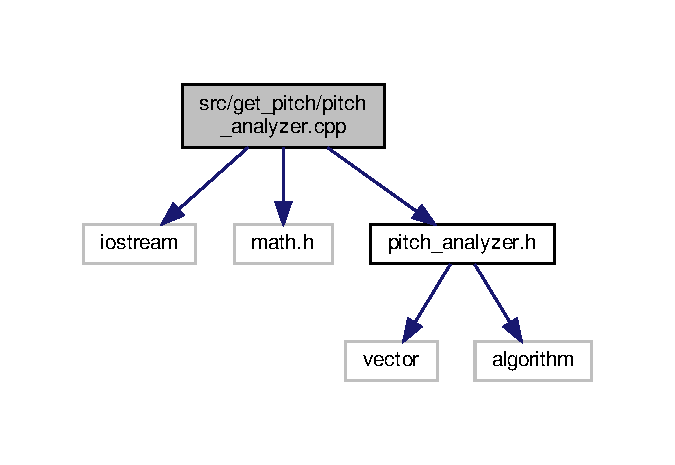
\includegraphics[width=324pt]{pitch__analyzer_8cpp__incl}
\end{center}
\end{figure}
\subsection*{Namespaces}
\begin{DoxyCompactItemize}
\item 
 \hyperlink{namespaceupc}{upc}
\begin{DoxyCompactList}\small\item\em Name space of U\+PC. \end{DoxyCompactList}\end{DoxyCompactItemize}

\hypertarget{pitch__analyzer_8h}{}\section{src/get\+\_\+pitch/pitch\+\_\+analyzer.h File Reference}
\label{pitch__analyzer_8h}\index{src/get\+\_\+pitch/pitch\+\_\+analyzer.\+h@{src/get\+\_\+pitch/pitch\+\_\+analyzer.\+h}}
{\ttfamily \#include $<$vector$>$}\newline
{\ttfamily \#include $<$algorithm$>$}\newline
Include dependency graph for pitch\+\_\+analyzer.\+h\+:
\nopagebreak
\begin{figure}[H]
\begin{center}
\leavevmode
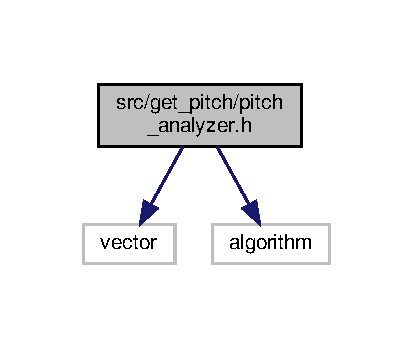
\includegraphics[width=198pt]{pitch__analyzer_8h__incl}
\end{center}
\end{figure}
This graph shows which files directly or indirectly include this file\+:
\nopagebreak
\begin{figure}[H]
\begin{center}
\leavevmode
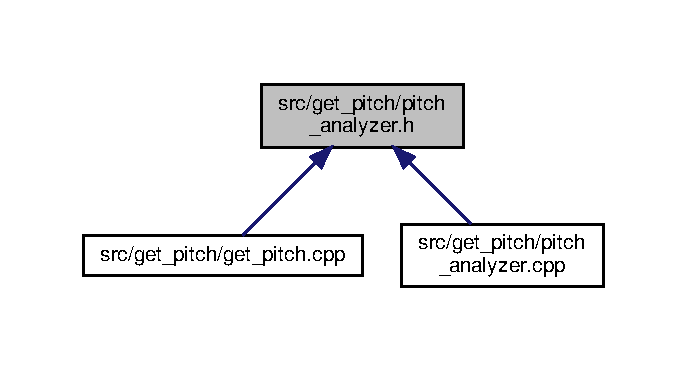
\includegraphics[width=330pt]{pitch__analyzer_8h__dep__incl}
\end{center}
\end{figure}
\subsection*{Classes}
\begin{DoxyCompactItemize}
\item 
class \hyperlink{classupc_1_1PitchAnalyzer}{upc\+::\+Pitch\+Analyzer}
\end{DoxyCompactItemize}
\subsection*{Namespaces}
\begin{DoxyCompactItemize}
\item 
 \hyperlink{namespaceupc}{upc}
\begin{DoxyCompactList}\small\item\em Name space of U\+PC. \end{DoxyCompactList}\end{DoxyCompactItemize}
\subsection*{Variables}
\begin{DoxyCompactItemize}
\item 
\mbox{\Hypertarget{namespaceupc_ae8ed4ce6dc2c05dfc1aa6432db41e1ae}\label{namespaceupc_ae8ed4ce6dc2c05dfc1aa6432db41e1ae}} 
const float \hyperlink{namespaceupc_ae8ed4ce6dc2c05dfc1aa6432db41e1ae}{upc\+::\+M\+I\+N\+\_\+\+F0} = 20.\+0F
\begin{DoxyCompactList}\small\item\em Minimum value of pitch in Hertzs. \end{DoxyCompactList}\item 
\mbox{\Hypertarget{namespaceupc_ab69be42753266b6e1a0deaa8eba56a19}\label{namespaceupc_ab69be42753266b6e1a0deaa8eba56a19}} 
const float \hyperlink{namespaceupc_ab69be42753266b6e1a0deaa8eba56a19}{upc\+::\+M\+A\+X\+\_\+\+F0} = 10000.\+0F
\begin{DoxyCompactList}\small\item\em Maximum value of pitch in Hertzs. \end{DoxyCompactList}\end{DoxyCompactItemize}

\hypertarget{pitch__evaluate_8cpp}{}\section{src/get\+\_\+pitch/pitch\+\_\+evaluate.cpp File Reference}
\label{pitch__evaluate_8cpp}\index{src/get\+\_\+pitch/pitch\+\_\+evaluate.\+cpp@{src/get\+\_\+pitch/pitch\+\_\+evaluate.\+cpp}}
{\ttfamily \#include $<$iostream$>$}\newline
{\ttfamily \#include $<$fstream$>$}\newline
{\ttfamily \#include $<$iomanip$>$}\newline
{\ttfamily \#include $<$vector$>$}\newline
{\ttfamily \#include $<$math.\+h$>$}\newline
{\ttfamily \#include $<$stdlib.\+h$>$}\newline
{\ttfamily \#include \char`\"{}docopt.\+h\char`\"{}}\newline
Include dependency graph for pitch\+\_\+evaluate.\+cpp\+:
\nopagebreak
\begin{figure}[H]
\begin{center}
\leavevmode
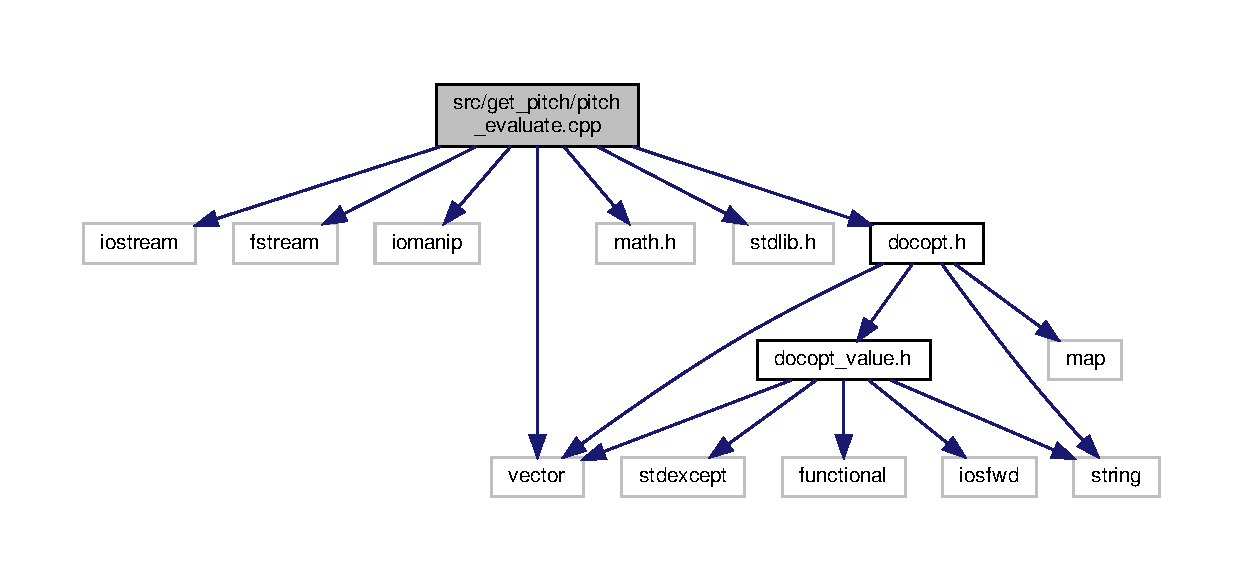
\includegraphics[width=350pt]{pitch__evaluate_8cpp__incl}
\end{center}
\end{figure}
\subsection*{Functions}
\begin{DoxyCompactItemize}
\item 
\mbox{\Hypertarget{pitch__evaluate_8cpp_acc47b8492bcbc1ad3fab7d6ac74d2d8d}\label{pitch__evaluate_8cpp_acc47b8492bcbc1ad3fab7d6ac74d2d8d}} 
int {\bfseries read\+\_\+vector} (const string \&filename, vector$<$ float $>$ \&x)
\item 
\mbox{\Hypertarget{pitch__evaluate_8cpp_a77944b5af41e256ec0ba1f00442cf9ba}\label{pitch__evaluate_8cpp_a77944b5af41e256ec0ba1f00442cf9ba}} 
void {\bfseries compare} (const vector$<$ float $>$ \&vref, const vector$<$ float $>$ \&vtest, int \&num\+\_\+voiced, int \&num\+\_\+unvoiced, int \&num\+\_\+voiced\+\_\+unvoiced, int \&num\+\_\+unvoiced\+\_\+voiced, int \&num\+\_\+voiced\+\_\+voiced, int \&num\+\_\+gross\+\_\+errors, float \&fine\+\_\+error)
\item 
\mbox{\Hypertarget{pitch__evaluate_8cpp_a6768ae9e20f3fec64eb692300953e0e0}\label{pitch__evaluate_8cpp_a6768ae9e20f3fec64eb692300953e0e0}} 
void {\bfseries print\+\_\+results} (int nframes, int num\+\_\+voiced, int num\+\_\+unvoiced, int num\+\_\+voiced\+\_\+unvoiced, int num\+\_\+unvoiced\+\_\+voiced, int num\+\_\+voiced\+\_\+voiced, int num\+\_\+gross\+\_\+errors, float fine\+\_\+errori, string filename)
\item 
\mbox{\Hypertarget{pitch__evaluate_8cpp_ac0f2228420376f4db7e1274f2b41667c}\label{pitch__evaluate_8cpp_ac0f2228420376f4db7e1274f2b41667c}} 
int {\bfseries main} (int argc, const char $\ast$argv\mbox{[}$\,$\mbox{]})
\end{DoxyCompactItemize}
\subsection*{Variables}
\begin{DoxyCompactItemize}
\item 
\mbox{\Hypertarget{pitch__evaluate_8cpp_ac3e1e3eb989b9766a74a68f946c1b20d}\label{pitch__evaluate_8cpp_ac3e1e3eb989b9766a74a68f946c1b20d}} 
const float {\bfseries gross\+\_\+threshold} = 0.\+2F
\end{DoxyCompactItemize}

%--- End generated contents ---

% Index
\backmatter
\newpage
\phantomsection
\clearemptydoublepage
\addcontentsline{toc}{chapter}{Index}
\printindex

\end{document}
